% Options for packages loaded elsewhere
\PassOptionsToPackage{unicode}{hyperref}
\PassOptionsToPackage{hyphens}{url}
%
\documentclass[
  12pt,
  a4paper,
  twoside]{article}
\usepackage{amsmath,amssymb}
\usepackage{setspace}
\usepackage{iftex}
\ifPDFTeX
  \usepackage[T1]{fontenc}
  \usepackage[utf8]{inputenc}
  \usepackage{textcomp} % provide euro and other symbols
\else % if luatex or xetex
  \usepackage{unicode-math} % this also loads fontspec
  \defaultfontfeatures{Scale=MatchLowercase}
  \defaultfontfeatures[\rmfamily]{Ligatures=TeX,Scale=1}
\fi
\usepackage{lmodern}
\ifPDFTeX\else
  % xetex/luatex font selection
\fi
% Use upquote if available, for straight quotes in verbatim environments
\IfFileExists{upquote.sty}{\usepackage{upquote}}{}
\IfFileExists{microtype.sty}{% use microtype if available
  \usepackage[]{microtype}
  \UseMicrotypeSet[protrusion]{basicmath} % disable protrusion for tt fonts
}{}
\makeatletter
\@ifundefined{KOMAClassName}{% if non-KOMA class
  \IfFileExists{parskip.sty}{%
    \usepackage{parskip}
  }{% else
    \setlength{\parindent}{0pt}
    \setlength{\parskip}{6pt plus 2pt minus 1pt}}
}{% if KOMA class
  \KOMAoptions{parskip=half}}
\makeatother
\usepackage{xcolor}
\usepackage[left=3.9cm, right=3.3cm, top=2.5cm, bottom=3cm]{geometry}
\usepackage{longtable,booktabs,array}
\usepackage{calc} % for calculating minipage widths
% Correct order of tables after \paragraph or \subparagraph
\usepackage{etoolbox}
\makeatletter
\patchcmd\longtable{\par}{\if@noskipsec\mbox{}\fi\par}{}{}
\makeatother
% Allow footnotes in longtable head/foot
\IfFileExists{footnotehyper.sty}{\usepackage{footnotehyper}}{\usepackage{footnote}}
\makesavenoteenv{longtable}
\usepackage{graphicx}
\makeatletter
\def\maxwidth{\ifdim\Gin@nat@width>\linewidth\linewidth\else\Gin@nat@width\fi}
\def\maxheight{\ifdim\Gin@nat@height>\textheight\textheight\else\Gin@nat@height\fi}
\makeatother
% Scale images if necessary, so that they will not overflow the page
% margins by default, and it is still possible to overwrite the defaults
% using explicit options in \includegraphics[width, height, ...]{}
\setkeys{Gin}{width=\maxwidth,height=\maxheight,keepaspectratio}
% Set default figure placement to htbp
\makeatletter
\def\fps@figure{htbp}
\makeatother
\setlength{\emergencystretch}{3em} % prevent overfull lines
\providecommand{\tightlist}{%
  \setlength{\itemsep}{0pt}\setlength{\parskip}{0pt}}
\setcounter{secnumdepth}{5}
% definitions for citeproc citations
\NewDocumentCommand\citeproctext{}{}
\NewDocumentCommand\citeproc{mm}{%
  \begingroup\def\citeproctext{#2}\cite{#1}\endgroup}
\makeatletter
 % allow citations to break across lines
 \let\@cite@ofmt\@firstofone
 % avoid brackets around text for \cite:
 \def\@biblabel#1{}
 \def\@cite#1#2{{#1\if@tempswa , #2\fi}}
\makeatother
\newlength{\cslhangindent}
\setlength{\cslhangindent}{1.5em}
\newlength{\csllabelwidth}
\setlength{\csllabelwidth}{3em}
\newenvironment{CSLReferences}[2] % #1 hanging-indent, #2 entry-spacing
 {\begin{list}{}{%
  \setlength{\itemindent}{0pt}
  \setlength{\leftmargin}{0pt}
  \setlength{\parsep}{0pt}
  % turn on hanging indent if param 1 is 1
  \ifodd #1
   \setlength{\leftmargin}{\cslhangindent}
   \setlength{\itemindent}{-1\cslhangindent}
  \fi
  % set entry spacing
  \setlength{\itemsep}{#2\baselineskip}}}
 {\end{list}}
\usepackage{calc}
\newcommand{\CSLBlock}[1]{\hfill\break\parbox[t]{\linewidth}{\strut\ignorespaces#1\strut}}
\newcommand{\CSLLeftMargin}[1]{\parbox[t]{\csllabelwidth}{\strut#1\strut}}
\newcommand{\CSLRightInline}[1]{\parbox[t]{\linewidth - \csllabelwidth}{\strut#1\strut}}
\newcommand{\CSLIndent}[1]{\hspace{\cslhangindent}#1}
\usepackage{booktabs}    % For table formatting
\usepackage{libertine}   % Font package (you can keep this as it is)
\usepackage{libertinust1math}  % Font package for math symbols (you can keep this as it is)
\usepackage{sourcecodepro}  % For source code font (you can keep this as it is)
\usepackage{emptypage}   % To remove the page numbers from empty pages (you can keep this as it is)
\usepackage{graphicx}    % For resizing tables to fit the text width
\usepackage{caption}     % For customizing caption alignment
\usepackage{longtable}   % For long tables spanning multiple pages
\usepackage{pdflscape}   % For landscape pages
\usepackage{rotating}    % For rotating tables (sideways tables)
\usepackage{geometry}    % For page layout customization
\usepackage{sectsty}      % To modify section styling

% Customize table settings
\renewcommand{\textfraction}{0.05}
\renewcommand{\topfraction}{0.8}
\renewcommand{\bottomfraction}{0.8}
\renewcommand{\floatpagefraction}{0.75}

% Resize tables to fit the text width and left-align captions, make them bold
\captionsetup{justification=raggedright, singlelinecheck=false,labelfont=bf}

% Optional: Change the font size for verbatim output
\let\oldverbatim\verbatim
\let\endoldverbatim\endverbatim
\renewenvironment{verbatim}{\footnotesize\oldverbatim}{\endoldverbatim}

\usepackage{pdfpages}

% titlesec does not play nice with RMarkdown, so hack:

\let\paragraph\oldparagraph
\let\subparagraph\oldsubparagraph
%\usepackage[sc, compact, raggedright]{titlesec}


\setlength{\parindent}{0.5in}
\setlength{\parskip}{0pt}
\usepackage{sectsty}
\sectionfont{\centering\bfseries\LARGE}
\subsectionfont{\bfseries\large}
\subsubsectionfont{\bfseries\itshape\large}
\ifLuaTeX
  \usepackage{selnolig}  % disable illegal ligatures
\fi
\usepackage{bookmark}
\IfFileExists{xurl.sty}{\usepackage{xurl}}{} % add URL line breaks if available
\urlstyle{same}
\hypersetup{
  pdftitle={Development of a German Instrument for Self-Rated Data Literacy},
  pdfauthor={Leonie Hagitte},
  hidelinks,
  pdfcreator={LaTeX via pandoc}}

\title{Development of a German Instrument for Self-Rated Data Literacy}
\usepackage{etoolbox}
\makeatletter
\providecommand{\subtitle}[1]{% add subtitle to \maketitle
  \apptocmd{\@title}{\par {\large #1 \par}}{}{}
}
\makeatother
\subtitle{An Algorithm-based Approach to Scale Development}
\author{Leonie Hagitte}
\date{2025-01-25}

\begin{document}
\maketitle

{
\setcounter{tocdepth}{2}
\tableofcontents
}
\setstretch{1.2}
\newpage\null\thispagestyle{empty}\newpage

\section*{Abstract}\label{abstract}
\addcontentsline{toc}{section}{Abstract}

This study aimed to develop a german, self-rated data literacy questionnaire tailored for non-specialized populations. Drawing on theoretical frameworks and previous operationalizations, the construct of data literacy was defined to include five facets: Comprehension, Evaluation, Integration, Communication, and Statistics. An initial pool of 71 items was refined through cognitive interviews and further narrowed to a final set of 20 items using an algorithm-based selection approach. Data were collected via a cross-sectional online survey (\emph{N} = 616), and the measurement model was assessed using confirmatory factor analysis (CFA). Model fit indices indicated acceptable fit (CFI = .96, SRMR = .08, RMSEA = .05) of the initial model. A multi-group CFA indicated deterioration of fit (CFI = .92, SRMR = .087, RMSEA = .038), but confirmed scalar invariance across subsamples (random sample split), indicating some stability of the measurement model. The scale exhibited acceptable internal consistency (McDonald's \(\omega\) = .92) and suggested criterion validity in most aspects, with moderate to strong correlations observed with constructs such as information literacy and need for cognition. In addition to the measurement properties, limitations were noted in factor independence due to multicollinearity among some facets, as well as due to correlated residuals of the scales items. The questionnaire provides the first step towards a novel tool for assessing data literacy in laypeople and warrants further research into the construct's structure, applications and relevance.

\emph{Keywords: Data Literacy, Questionnaire Development, Algorithm-Based Item Selection, Genetic Algorithm}

\section*{Acknowledgements}\label{acknowledgements}
\addcontentsline{toc}{section}{Acknowledgements}

I want to thank my advisers, Prof.~Martin Schultze, Prof.~Timo Lorenz, and Prof.~Manuel Völkle for their time and patience, and my friends for their resourceful advice.

\newpage\null\thispagestyle{empty}\newpage

\section{Background}\label{background}

In a world characterized by information overload and rapid technological advancements (\citeproc{ref-Koltay2017}{Koltay, 2017}; \citeproc{ref-Leighton2021}{Leighton et al., 2021}; \citeproc{ref-Roetzel2019}{Roetzel, 2019}), the relevance of data literacy for today's society becomes evident. Data literacy serves as a potent tool in navigating the complex data-driven environment (\citeproc{ref-Carmi2020}{Carmi et al., 2020}; \citeproc{ref-Cui2023}{Cui et al., 2023}; \citeproc{ref-Leighton2021}{Leighton et al., 2021}; \citeproc{ref-risdale2015}{Ridsdale et al., 2015}) and individuals equipped with strong data literacy skills can discern patterns, critically evaluate information, and make informed decisions (\citeproc{ref-Chen2024}{F. Chen et al., 2024}; \citeproc{ref-Cui2023}{Cui et al., 2023}).
The exploration of citizens' interaction with media and the cultivation of their agency has traditionally started around concepts such as written literacy and information literacy (\citeproc{ref-ACRL2000}{Association of College \& Research Libraries, 2000}; \citeproc{ref-brown2002}{C. Brown \& Krumholz, 2002}). Information literacy, as defined by the American Library Association in 1989, encompasses the skills required to locate, evaluate, and effectively use information (\citeproc{ref-brown2002}{C. Brown \& Krumholz, 2002}). This foundational understanding of information literacy has evolved through various frameworks and models, emphasizing its importance in educational settings and lifelong learning (\citeproc{ref-tomar2023}{Tomar, 2023}). In more recent discussions, data literacy has been approaching relevance among discussed competencies regarding agency in the current society (\citeproc{ref-Carmi2020}{Carmi et al., 2020}; \citeproc{ref-Leighton2021}{Leighton et al., 2021}). Deficiency in data literacy not only exposes individuals to various risks and harms on personal, social, physical, and financial levels but also constrains their capacity to actively engage as informed citizens within an evolving, data-driven society (\citeproc{ref-Carmi2020}{Carmi et al., 2020}; \citeproc{ref-Leighton2021}{Leighton et al., 2021}). Thus, data literacy is a competency that is becoming increasingly important to everyone. Research has acknowledged this in recent years, as more and more has been undertaken in that direction (\citeproc{ref-Chen2024}{F. Chen et al., 2024}; \citeproc{ref-Cui2023}{Cui et al., 2023}). This study aims to complement the current research, with a self rating questionnaire for assessing data literacy among citizens.

Data literacy involves the ability to effectively collect, manage, evaluate, and apply data in a critical manner (\citeproc{ref-risdale2015}{Ridsdale et al., 2015}). According to Wolff et al. (\citeproc{ref-wolff2016}{2016}), it means being able to ask and answer everyday questions using both small and large datasets while considering ethical aspects. This includes skills such as selecting, cleaning, analyzing, visualizing, criticizing, and interpreting data, as well as communicating insights from data, and using data for various purposes. Frank et al. (\citeproc{ref-frank2016}{2016}) distinguishes between cognitive skills, like data collection and analysis, and social skills, which involve trusting data while maintaining skepticism. Calzada-Prado \& Marzal (\citeproc{ref-prado2013}{2013}) outline five dimensions of data literacy: understanding data, acquiring data, interpreting and evaluating data, managing data, and using data. Understanding data includes knowing their types, roles, and significance, while acquiring data involves evaluating and selecting sources. Interpreting and evaluating data encompass understanding different presentation methods and data interpretation. Managing data includes storage, management, and re-use. Using data involves preparation, analysis, communication, and ethical considerations (\citeproc{ref-prado2013}{Calzada-Prado \& Marzal, 2013}).
This small comparison already highlights one prominent attribute of data literacy: it is a heterogeneous concept (\citeproc{ref-Chen2024}{F. Chen et al., 2024}). Every subject or profession seems to hold their own definition or framework of data literacy (\citeproc{ref-Chen2024}{F. Chen et al., 2024}; \citeproc{ref-Cui2023}{Cui et al., 2023}). While heterogeneity is beneficial for assessing specific skills (e.g.~in a recruitment test), it limits the generalisability and comparability of data literacy across individuals with different background. It furthermore limits the accuracy of communication about the topic as two people with different background might hold different definitions on data literacy. In the study of Cui et al. (\citeproc{ref-Cui2023}{2023}) it also becomes apparent, that one group seems to be less focused on in the research on data literacy: citizens or the broader public. Citizens in this case mean people of the general public, that hold no special role or profession, related to data handling or aspects related to data literacy (\citeproc{ref-wolff2016}{Wolff et al., 2016}).
Despite being the largest demographic group, citizens are often overlooked in favor of specific professions such as researchers, librarians, students, or educators (\citeproc{ref-Cui2023}{Cui et al., 2023}). This trend raises questions about the emphasis on certain aspects of data literacy, many of which tend to align more closely with professional roles than with the needs of laypeople (\citeproc{ref-schuxfcller2020}{Schüller, 2020}).
In their framework Schüller (\citeproc{ref-schuxfcller2020}{2020}) highlight the different roles, people can hold: Some of the factors or skills regard \emph{data-consumption}, whereas the most are skills \emph{data-producers} would have. This is also reflected when taking a look into related concepts. The definition proposed by Wolff et al. (\citeproc{ref-wolff2016}{2016}) suggests that data literacy shares some common competencies with statistical and information literacies.\\
Information literacy, often studied in library sciences, overlaps with data literacy in terms of accessing, critically evaluating, and using data sources (\citeproc{ref-prado2013}{Calzada-Prado \& Marzal, 2013}; \citeproc{ref-shields2005}{Shields, 2005}). Wolff et al. (\citeproc{ref-wolff2016}{2016}) also emphasize the importance of the data inquiry process, starting from identifying problems, designing studies, acquiring data, conducting analysis, to drawing data-based conclusions. In comparison, Gould (\citeproc{ref-gould2017}{2017}) argued that data literacy is essentially the same as statistical literacy but with additional competencies needed due to the increasing importance of data. These added competencies include understanding who collects the data, how and why data is collected, and understanding data privacy and ownership (\citeproc{ref-gould2017}{Gould, 2017}).

Additionally, when discussing data literacy, it is essential to understand the distinctions between the terms data and information, and their relationship to one another. The concepts of data and information are foundational in various fields, yet their precise definitions and relationships are often subject to interpretation (\citeproc{ref-Koltay2017}{Koltay, 2017}; \citeproc{ref-Schneider2013}{R. Schneider, 2013}). While data can be viewed as the raw material (\citeproc{ref-shannon1948}{Shannon, 1948}) from which information is derived (\citeproc{ref-bates2009}{Bates, 2009}), it is the reduction of entropy through organization and interpretation that gives rise to meaningful information (\citeproc{ref-brillouin1953}{Brillouin, 1953}; \citeproc{ref-jaynes1957}{Jaynes, 1957}). Thus, rather than viewing data as synonymous with entropy or information, it is more accurate to consider information as emerging from the structured representation of data.

It is structured representation of data, that also according to the framework of (\citeproc{ref-schuxfcller2020}{Schüller, 2020}), citizens are primarily concerned with: citizens are holding roles where they mainly consume data or information. Consequently, they may encounter difficulties with tasks or items related to producing facets such as providing or exploiting data. This imbalance could potentially undermine the fairness of tests and questionnaires designed to assess data literacy, particularly, if these assessments prioritize competencies closer to data and statistical literacy over those closer to information literacy.

\subsection{Conceptual Integration and Delineation From Other Concepts}\label{conceptual-integration-and-delineation-from-other-concepts}

Because data literacy is such a heterogeneous construct, it is very prone to construct proliferation. This, for example, becomes evident, when looking into the literature review from Cui et al. (\citeproc{ref-Cui2023}{2023}). In their study they found over fourteen different definitions of data literacy, incorporating different sets of 75 competencies. Furthermore, very few of those definitions are targeted at citizens, and none of the questionnaires they report target citizens.
Thus, the objective of the present study was to formulate a definition of data literacy, based on the current literature, that works for citizens. For the conceptual integration, I used the review of Cui et al. (\citeproc{ref-Cui2023}{2023}) and assessed what competencies were incorporated in most of the definitions, and would therefore be considered central to the construct. This included counting the same competencies as well as checking what competencies might be named differently, but are considered the same substantively. Furthermore, data literacy encompasses certain characteristics and behaviors from similar constructs. Examples for those convergent constructs are \emph{critical thinking}, \emph{media competency}, \emph{technology competency}, \emph{statistical literacy} as well as \emph{information literacy} (\citeproc{ref-Chen2024}{F. Chen et al., 2024}; \citeproc{ref-Cui2023}{Cui et al., 2023}; \citeproc{ref-Leighton2021}{Leighton et al., 2021}). As those constructs share substantive parts, differing in size regarding the respective definition of the constructs, it is to be expected that all of them show moderate to strong positive correlations.
Concluding, data literacy can be defined as ``the ability to collect, manage, evaluate, and apply data effectively. It involves asking and answering real-world questions from datasets while considering ethical use. Core skills include selecting, cleaning, analyzing, visualizing, presenting, critiquing, and interpreting data, information and their sources'' (\citeproc{ref-Cui2023}{Cui et al., 2023}; \citeproc{ref-risdale2015}{Ridsdale et al., 2015}; \citeproc{ref-wolff2016}{Wolff et al., 2016}).

Most definitions in the literature discern about five factors of general data literacy (\citeproc{ref-Cui2023}{Cui et al., 2023}), which can be further categorized into three \emph{consumer} and two \emph{producer} facets (\citeproc{ref-schuxfcller2020}{Schüller, 2020}). Trying to describe the associated behaviors, I labeled these five factors as \emph{Comprehension}, \emph{Evaluation}, \emph{Integration}, \emph{Communication}, and \emph{Statistics}. The \emph{consumer} facets: \emph{Comprehension}, \emph{Evaluation}, and \emph{Integration}, are broadly relevant to nearly everyone in society, including the general public. In contrast, the \emph{producer} facets: \emph{Communication} and \emph{Statistics}, are primarily important for individuals actively working with data. The \emph{consumer} facets are closely aligned with media literacy, emphasizing critical analysis and interpretation of various media formats to support understanding and engagement with media content (cf.~Table 1).

\begin{table}[!htbp]
\centering
\caption{The Nomological Network of the Construct and its Factors}
\scriptsize
\begin{tabular}{|p{0.15\textwidth}|p{0.30\textwidth}|p{0.25\textwidth}|p{0.21\textwidth}|}
\hline
\textbf{Factor} & \textbf{Description} & \textbf{Convergent Constructs} & \textbf{Adjacent Constructs} \\
\hline
\textbf{Data Literacy} & The ability to collect, manage, evaluate, and apply data effectively. & Statistical Literacy +++

Information Literacy +++

Media Competency ++

Critical Thinking ++
& Need for Cognition +

Openness +

Conscientiousness + \\
\hline
\textbf{Comprehension} & Individuals with high scores on this factor demonstrate a strong aptitude for processing and making sense of information across different formats, enabling them to draw accurate conclusions and insights. & Statistical Literacy ++

Information Literacy +++

Media Competency ++

Critical Thinking +++
& Need for Cognition: +

Openness +

Conscientiousness +\\
\hline
\textbf{Evaluation} & Represents the ability to evaluate the credibility and reliability of information by considering the reputation of the source, the context in which it is presented, and potential biases or vested interests. Individuals high in this factor demonstrate a heightened awareness of these elements. & Statistical Literacy ++

Information Literacy +++

Media Competency +++

Critical Thinking +
& Need for Cognition: ++ 

Openness +

Conscientiousness +\\
\hline
\textbf{Integration} & Reflects the ability to seek a comprehensive understanding of diverse topics by engaging with multiple perspectives and integrating data-driven insights. Individuals high in this factor are open to adapting their opinions based on new evidence, prioritize evidence-based information, and strive to align their values with reliable data. & Statistical Literacy ++

Information Literacy ++

Media Competency ++

Critical Thinking +++ 
& Need for Cognition: ++ 

Openness ++

Conscientiousness +\\
\hline
\textbf{Communication} & Individuals scoring high in this factor hold the ability to translate data into simple visualizations, present findings confidently, and articulate complex information effectively in written and visual as well as verbal formats. & Statistical Literacy +++

Information Literacy ++

Media Competency +++

Critical Thinking ++
& Need for Cognition: +

Openness +

Conscientiousness +\\
\hline
\textbf{Statistics} & It involves proficiency in organizing and analyzing data using software tools, conducting statistical analyses, and understanding research methodologies. & Statistical Literacy +++

Information Literacy ++

Media Competency ++

Critical Thinking +
& Need for Cognition: ++ 

Openness +

Conscientiousness ++\\
\hline
\end{tabular}
\begin{flushleft}
\vspace{9pt}
\footnotesize\textit{Note}. The table illustrates the nomological network of Data Literacy and its factors. Each factor is described in terms of its primary function, along with convergent constructs and adjacent constructs. The constructs are displayed alongside their expected correlation with the data literacy factors (+++ = strong positive, ++ = moderate positive, + = weak positive).    
\end{flushleft}

\end{table}

\subsubsection{Consumer Facets}\label{consumer-facets}

The factor \emph{Comprehension} encompasses behaviors and skills associated with critical thinking (\citeproc{ref-payan2022}{Payan Carreira et al., 2022}; \citeproc{ref-rear2019}{Rear, 2019}), such as identifying weaknesses in ones reasoning or actively shaping discourse and public dissemination of information. It involves the ability to comprehend various forms of data presentation, detect inconsistencies, interpret data comprehensively, and identify logical fallacies. Individuals with high scores on this factor demonstrate a strong aptitude for processing and making sense of information across different formats, enabling them to draw accurate conclusions and insights (\citeproc{ref-carlson2014}{Carlson et al., 2014}; \citeproc{ref-vahey2006}{Vahey et al., 2006}; \citeproc{ref-wolff2016}{Wolff et al., 2016}).
Both statistical and information literacy involve using data, and information to make informed decisions (\citeproc{ref-callingham2006}{Callingham, 2006}; \citeproc{ref-Gal2002}{Gal, 2002}; \citeproc{ref-Webber2017}{Webber \& Johnston, 2017}).
Therefore, the \emph{Evaluation} factor involves skills related to critically evaluating information sources and discerning between facts and opinions (\citeproc{ref-callingham2006}{Callingham, 2006}; \citeproc{ref-frank2016}{Frank et al., 2016}; \citeproc{ref-gould2017}{Gould, 2017}; \citeproc{ref-kouts-klemm2019}{Kõuts-Klemm, 2019}).
It includes elements of information literacy (\citeproc{ref-ACRL2000}{Association of College \& Research Libraries, 2000}) by focusing on evaluating the credibility of data sources, considering factors like reputation and biases, similar to assessing the quality of information sources (Evaluation \& Integration) (\citeproc{ref-Webber2017}{Webber \& Johnston, 2017}).
Individuals scoring high on this factor demonstrate awareness of potential biases or vested interests in information sources, as well as the context in which the information was presented (\citeproc{ref-callingham2006}{Callingham, 2006}; \citeproc{ref-kouts-klemm2019}{Kõuts-Klemm, 2019}; \citeproc{ref-lusiyana2020}{Lusiyana et al., 2020}).

Data literacy often emphasizes integrating data-driven insights into one's opinions and values, which influence decision-making processes, without focusing on the decision making (\citeproc{ref-callingham2006}{Callingham, 2006}; \citeproc{ref-wolff2016}{Wolff et al., 2016}). Thereby it aligns with the goals of statistical and information literacy (cf.~Table 1).
The \emph{Integration} factor relates to the ability and motivation to integrate data-driven insights into one's worldview and values (\citeproc{ref-callingham2006}{Callingham, 2006}; \citeproc{ref-Carmi2020}{Carmi et al., 2020}; \citeproc{ref-wolff2016}{Wolff et al., 2016}). It involves actively seeking comprehensive understanding of various topics, engaging with diverse perspectives, and consciously incorporating data-driven insights. Individuals scoring high in this factor adapt their opinions based on new data, prefer evidence-based information, and ensure their values align with reliable data. They engage with information and perspectives that challenge their existing views, showing a willingness to reassess their opinions and positions based on new data (\citeproc{ref-Carmi2020}{Carmi et al., 2020}).

\subsubsection{Producer Facets}\label{producer-facets}

The \emph{Communication} factor revolves around the often referenced skill to effectively communicate and present data through various means, including visual formats, verbal explanations, and written descriptions (\citeproc{ref-prado2013}{Calzada-Prado \& Marzal, 2013}; \citeproc{ref-kouts-klemm2019}{Kõuts-Klemm, 2019}; \citeproc{ref-wolff2016}{Wolff et al., 2016}).
It requires translating complex data into clear formats, ensuring comprehension by varied audiences. Individuals scoring high in this factor hold the ability to translate data into simple visualizations, present findings confidently, and articulate complex information effectively in written, visual as well as verbal formats (\citeproc{ref-prado2013}{Calzada-Prado \& Marzal, 2013}; \citeproc{ref-kouts-klemm2019}{Kõuts-Klemm, 2019}; \citeproc{ref-wolff2016}{Wolff et al., 2016}).

This definition, incorporates statistical literacy by emphasizing data interpretation, analysis, and understanding different types of data representations, such as graphs and tables (Statistics) (\citeproc{ref-Gal2002}{Gal, 2002}).
The \emph{Statistics} factor covers skills related to managing and analyzing data effectively (\citeproc{ref-gould2017}{Gould, 2017}; \citeproc{ref-risdale2015}{Ridsdale et al., 2015}). It involves proficiency in organizing and analyzing data using software tools, conducting statistical analyses, and understanding research methodologies (\citeproc{ref-gould2017}{Gould, 2017}; \citeproc{ref-williams2014}{Williams et al., 2014}). Individuals scoring high on this factor exhibit competence in conducting interviews or surveys for data collection, performing basic statistical analysis and recognizing trends in graphical representations (\citeproc{ref-deahl2014}{Deahl, 2014}; \citeproc{ref-gould2017}{Gould, 2017}; \citeproc{ref-williams2014}{Williams et al., 2014}). In contrast to this presented concept of the \emph{Statistics} factor, statistical literacy often focuses more narrowly on statistical concepts and methods, such as probability, sampling, and hypothesis testing (\citeproc{ref-Gal2002}{Gal, 2002}; \citeproc{ref-gould2017}{Gould, 2017}). The \emph{Statistics} factor encompasses a broader range of skills beyond statistical concepts, such as data visualization, software usage, and understanding data collection methods. While information literacy involves assessing the quality of information sources, this data literacy definition places a particular emphasis on assessing data quality, considering factors like sample size, biases, and data context. This aspect extends beyond traditional information literacy (\citeproc{ref-ACRL2000}{Association of College \& Research Libraries, 2000}) and is more specific to data literacy.\\
The factors \emph{Evaluation} and \emph{Statistics} encompass behaviors and skills related to digital competency, including navigating and critically evaluating online sources and platforms, using information and communication technology (ICT), and utilizing statistical software. While digital competency focuses on the operational aspects of digital tools (\citeproc{ref-Zhao2021}{Zhao et al., 2021}), data literacy emphasizes the critical evaluation and application of data within specific contexts.

\subsection{Nomological net}\label{nomological-net}

The term data literacy could evoke associations with skills, abilities or knowledge.
Ability refers to an individuals potential or aptitude, encompassing innate or developed capacities across domains such as linguistic, mathematical, or motor abilities (\citeproc{ref-carroll1993}{Carroll, 1993}).
Knowledge, by contrast, is the cognitive representation or mental model of information, objects, and relationships. It forms the informational basis for interaction with and interpretation of the environment, encompassing all stored and retrievable data within an individuals mental framework (\citeproc{ref-NormanRumelhart1975}{Norman \& Rumelhart, 1975}).
Skill describes the application of learned and task-specific activities, often categorized into motor, cognitive, or social domains. Unlike abilities, skills imply mastery achieved through practice and are typically assessed based on performance quality (\citeproc{ref-green1998}{Green, 1998}).

Motivational theories have evolved from broad mechanistic views to more nuanced understandings that incorporate social-cognitive aspects of motivation, highlighting the interplay between personality traits and learning outcomes (\citeproc{ref-dweck1988}{Dweck \& Leggett, 1988}; \citeproc{ref-mischel1973}{Mischel, 1973}; \citeproc{ref-ross2005}{Ross et al., 2005}).
This reflects a broader trend in psychology where the understanding of learning is increasingly contextualized within the individual learners psychological profile, including their personality characteristics (\citeproc{ref-elander2004}{Elander, 2004}; \citeproc{ref-komarraju2011}{Komarraju et al., 2011}; \citeproc{ref-mischel1973}{Mischel, 1973}).
Those constructivist theories advocate for learning as a socially mediated process, where personality traits such as openness to experience and conscientiousness can significantly influence how learners engage with content and interact with peers (\citeproc{ref-komarraju2011}{Komarraju et al., 2011}).

The role of motivation, influenced by personality traits, is particularly relevant in the context of competencies such as data literacy.
Data literacy requires not only cognitive skills but also the motivation to engage with data, interpret it, and apply it effectively (\citeproc{ref-keshavarz2021}{Keshavarz, 2021}).
Research indicates that individuals with high levels of conscientiousness and openness are more likely to pursue learning opportunities related to data literacy, as these traits correlate with intrinsic motivation and a proactive approach to learning (\citeproc{ref-keshavarz2021}{Keshavarz, 2021}; \citeproc{ref-mahmood2021}{Mahmood et al., 2021}; \citeproc{ref-saleh2018}{Saleh et al., 2018}).
For example, students who exhibit high conscientiousness tend to set specific learning goals and persist in their efforts to achieve them, which is essential for mastering complex skills like data analysis (\citeproc{ref-komarraju2009}{Komarraju et al., 2009}; \citeproc{ref-saleh2018}{Saleh et al., 2018}).\\
Thus, data literacy can be seen as more on the side of proficiencies, because many behaviors incorporated in data literacy go beyond the mere question of whether a person is `able to do it'. It includes the question of one's motivation to do it.

\subsubsection{Need for Cognition}\label{need-for-cognition}

The concept of \emph{Need for Cognition} (NFC), can be defined as ``a need to structure relevant situations in meaningful, integrated ways. It is a need to understand and make reasonable the experiential world'' (\citeproc{ref-cohen1955}{Cohen et al., 1955, p. 291}). The concept captures individual variations in the engagement and enjoyment of thinking tasks (\citeproc{ref-bless1994}{Bless et al., 1994}). As data literacy incorporates several cognitive aspects as well as the motivation to understand data and information one gets presented with, it is expected to correlate positively with NFC. As NFC is more trait-like and data literacy is more a competency and therefore less stable, a small, nonetheless positive correlation is expected (i.e.~correlation should be small) (cf.~Table 1).

\subsubsection{Opennes to new Experiences}\label{opennes-to-new-experiences}

\emph{Openness to new experiences} is one factor of the \emph{Big Five} (\citeproc{ref-costa1992}{Costa \& McCrae, 1992}) and reflects a broad appreciation for art, emotion, adventure, unconventional ideas, imagination, curiosity, and diverse experiences (\citeproc{ref-john2008}{John et al., 2008}). Individuals high in openness tend to be intellectually curious, receptive to emotions, appreciative of beauty, and eager to explore new possibilities. They are often more creative and emotionally attuned compared to those low in openness. In contrast, individuals low in openness tend to seek fulfillment through perseverance and are characterized as pragmatic and sometimes viewed as dogmatic or closed-minded (\citeproc{ref-john2008}{John et al., 2008}). As already mentioned, data literacy can be thought of as a competency, thus incorporating the individual motivation, leading to a certain behavior. Therefore, openness to new experiences is expected to correlate positively with data literacy. As openness to new experiences is more trait-like and data literacy is not, the correlation is expected to be small (cf.~Table 1).

\subsubsection{Conscientiousness}\label{conscientiousness}

\emph{Conscientiousness} is one factor of the \emph{Big Five} (\citeproc{ref-costa1992}{Costa \& McCrae, 1992}) and refers to an individuals propensity for self-discipline, dutifulness, and striving for achievement in alignment with external standards or expectations. It encompasses levels of impulse control, regulation, and goal-directed behavior (\citeproc{ref-costa1992}{Costa \& McCrae, 1992}; \citeproc{ref-john2008}{John et al., 2008}; \citeproc{ref-toegel2012}{Toegel \& Barsoux, 2012}). High conscientiousness is characterized by persistence and focus, often perceived as stubbornness, whereas low conscientiousness is linked to flexibility and spontaneity, potentially manifesting as carelessness and unreliability (\citeproc{ref-toegel2012}{Toegel \& Barsoux, 2012}). Individuals with high conscientiousness tend to prefer planned actions over spontaneous ones (\citeproc{ref-costa1992}{Costa \& McCrae, 1992}; \citeproc{ref-john2008}{John et al., 2008}).\\
The cognitive aspects of data literacy as well as the motivation to understand data and information speaks to the conscientiousness of people as well. As being critical and at times detail oriented (e.g.~in interpreting results, or spotting inconsistencies in presented information or while examining the credibility of sources) is also integral to data literacy, they are are expected to correlate positively. However, as conscientiousness is expected to be more stable over time, opposing to data literacy, a small, nonetheless positive correlation is expected (i.e.~correlation should be small) (cf.~Table 1).

\subsection{Aim of the Study}\label{aim-of-the-study}

The aim was to derive a comprehensive definition of data literacy based on existing approaches and to develop a questionnaire for self-rated data literacy with citizens being the target population. Thus the research question of this study is:

\noindent ``Does the proposed set of items effectively capture the latent factor structure of self-rated data literacy, and can the created scale be considered a reliable and valid measure of this construct?''

\noindent \textit{H1: The training-data will support the suggested latent factor structure and the proposed measurement model.}\\
\emph{H2: The latent factor structure of the initial analysis will be supported by a different sample.}\\
\emph{H3: A moderate to high positive correlation with information behavior related self-efficacy (SWE-IV-16) (\citeproc{ref-behm2018}{Behm, 2018}) is expected.}\\
\emph{H4: A moderate positive correlation with self-perceived competence in using information and communication technology (ICT-SC25) (\citeproc{ref-schauffel2021}{Schauffel et al., 2021}) is expected.}\\
\emph{H5: A small positive correlation with need for cognition (NFC-K) (\citeproc{ref-beiuxdfert2015}{Beißert et al., 2015}) is expected.}\\
\emph{H6: A small positive correlation with openness to new experiences (BFI-10) (\citeproc{ref-rammstedt2014}{Rammstedt et al., 2014}) is expected.}\\
\emph{H7: A small positive correlation with conscientiousness (BFI-10) (\citeproc{ref-rammstedt2014}{Rammstedt et al., 2014}) is expected.}

\section{Methods}\label{methods}

\subsection{Item Creation}\label{item-creation}

Prior to the item creation, a review of the literature was done. Since the goal was to create a self-report questionnaire, the indicators of the latent constructs were decided to be subjective indicators, or \emph{Q-data} (\citeproc{ref-buehner2021}{Bühner, 2021}). Furthermore it was set that the target group for the questionnaire are German speaking citizens. There were no clear restrictions regarding age or education, other than the participants being of legal age and that the questionnaire should not be directed at professionals in terms of data literacy, or highly educated people.

The item creation itself was oriented towards the Act-Frequency-Approach (\citeproc{ref-buss1983}{Buss \& Craik, 1983}), thus the prototype approach.
I started with thinking of frequent, relevant behaviors, convictions or believes reflecting the factors of data literacy, hence being prototypical of those latent factors.
For the \emph{Comprehension} factor that could be recognizing whether the interpretations of others fit the available data, or recognizing when one is presented with contradictory information or understand the information a graphic contains, when data is presented visually.
Regarding the \emph{Evaluation} factor that could be assessing the credibility of information, or consider the reputation of the source. As well as being aware that publishers' own interests can influence the published information or to check information by comparing several sources with each other.
The \emph{Integration} factor could be represented by dealing with information that challenges ones views or consciously incorporating data-based findings into ones opinion-forming process. Additionally it could also manifest itself in changing ones mind if new data calls it into question.
For the \emph{Communication} factor, that could be represented by feeling confident in presenting data in visual formats in a way that can be understood by different target groups. But also to feel confident in expressing ones point of view in discussions or being able to summarize the most important information from data sets.
As for the \emph{Statistics} factor, this could be represented by knowing how to distinguish between causality and correlation or analyzing data sets using simple statistical methods.

That way, over 100 potential items have been created, that were then refined in terms of wording, structure but content as well.
I avoided inversely worded items, and decided to not ask for specific examples, because those might enhance the difficulty of the respective items, depending on the personal background of the person answering the question.
Additionally, I made sure that items were only ever asking for one behavior, conviction or opinion at once.
Overall I tried to formulate the items as easy and understandable as possible.
Ten cognitive interviews were held to refine those potential items, and to confirm the prototypicality of the behaviors etc. asked in the items.
The cognitive interviews comprised the think-aloud technique as well as probing, to get an understanding of how the items are perceived, what comes to mind when reading the items and whether the items really ask for relevant behaviors (\citeproc{ref-fowler1995}{Fowler, 1995}). Furthermore, that way unclear formulations or difficult wordings could be resolved.
The interviews were administered iteratively to refine the items consecutively.
In the interviews it became apparent, that especially the degree to which people can relate to the factors four and five differed heavily. This was expected, since those producer factors are considered to play a lesser role in the every day live of citizens. It also turned out that some words like \emph{data}, \emph{source} or \emph{information} are understood differently regarding the personal background.
The ages of the interview participants ranged from 21 to 66 years. Among the ten participants, three were men and seven were women. Their professional backgrounds included diverse occupations: students, an employee at a sports facility, a music teacher, an IT professional, a civil servant, a construction manager, and two nurses (one working in an intensive care unit and the other in an operating unit). Additionally, two of the participants were retired.
After the cognitive interviews of the 118 potential items, 71 remained.

\subsection{Sample}\label{sample}

The participants were recruited through a combination of personal and professional networks, along with outreach on several online social media platforms (e.g.~\emph{Instagram}, \emph{LinkedIn}, \emph{Whatsapp}, \emph{Telegram} and via e-mail). Conducted in German, the participation in the study was entirely voluntary, with no external incentives provided. An a-priori power analysis was conducted to determine the necessary sample size for the structural equation modelling. I used the `semPower' package in R (\citeproc{ref-moshagen2024}{Moshagen \& Bader, 2024}) and also took a look into studies with similar goals and methods.
The power analysis gave an analytical estimate of \emph{N} = 645, and a simulated estimate \emph{N} = 613, for the respective measurement model.
In the literature sample sizes of \emph{N} = 500 up to \emph{N} = 1000 could be found (\citeproc{ref-algner2022}{Algner \& Lorenz, 2022}; \citeproc{ref-remmert2022}{Remmert et al., 2022}; \citeproc{ref-schneider2024}{J. Schneider et al., 2024}).
Accordingly, the target sample size for this study was selected to fall within this range, to balance practical feasibility with theoretical recommendations.

Participants had to be of legal age to be included in the study. Furthermore, attention check questions were included (three instructed response items and one seriousness check item at the end) within the survey to assess participants' attentiveness. Participants who failed to correctly answer two out of the four attention check questions were excluded from the analysis.

\subsubsection{Demographics}\label{demographics}

The following characteristics of this study's sample are being made with referral to the respective statistics in the German population of 2022 (\citeproc{ref-BfA2024}{Bundesargentur für Arbeit, 2024}; \citeproc{ref-StBA2023a}{Statistisches Bundesamt, 2023a}, \citeproc{ref-StBA2023b}{2023b}, \citeproc{ref-StBA2024a}{2024c}, \citeproc{ref-StBA2024b}{2024b}, \citeproc{ref-StBA2024c}{2024a}).
The sample for this study comprised \emph{N} = 616 participants. Within the sample, 48.3\% identified as female (50.65\%), 50.2\% as male (49.35\%), and 1.5\% did not identify with binary gender categories. The average age was 40 years (\emph{M} = 44.6), with an average age of 39 years (\emph{M} = 38.79; \emph{SD} = 14.5) amongst women (\emph{M} = 45.9) and 42 years (\emph{M} = 41.96; \emph{SD} = 14.23) amongst men (\emph{M} = 43.2). The average age of people not identifying with binary gender was 28 years (\emph{M} = 27.63; \emph{SD} = 11.0).
Regarding education, 31.9\% of the participants reported a university degree as their highest educational level, 19.6\% reported a degree from a university of applied sciences, 18.0\% of the participants reported A-levels and 12.8\% of the participants reported a completed apprenticeship as their highest educational level. The remaining participants were distributed across the other categories.
Among participants who reported being employed, 64.88\% indicated full-time employment.
Specifically, 51.75\% of women and 77.73\% of men reported full-time employment at the time (65.15\%; men: 42.40\%, women: 22.75\%).
In contrast, 35.12\% of all employed participants reported working part-time.
At the time of the survey, 48.25\% of women and 22.27\% of men reported working part-time (28.22\%;men = 6.16\%; women = 22.06\%).
Additionally, 13.52\% of all participants indicated that they were not employed at the time (6.63\%).
The study encompassed every sector within the occupational classification at least once. 25.2\% of the participants indicated that they were students at the time of the survey (3.39\%).

\subsection{Open Science Standards}\label{open-science-standards}

This project used the reproducibility workflow proposed by Peikert et al. (\citeproc{ref-Peikert2021}{2021}). `Docker' and `renv' work together to create a reproducible and portable environment. `Docker' captures the complete software stack, while `renv' focuses on
managing R package dependencies and providing a clear documentation of the R
package environment. This combination ensures that the analysis can be easily
reproduced and shared with others in a reliable and transparent manner.
The study, including all associated code, has been made openly available on GitHub as part of the commitment to open science. The repository can be accessed at \url{https://github.com/LeonieHagitte/Thesis}.
The whole text is also hosted on GitHub-pages \url{https://leoniehagitte.github.io/Thesis/}.
It is to be mentioned, that the `repro' package from Peikert et al. (\citeproc{ref-Peikert2021}{2021}) has slightly changed in its functionality, namely that it does not ensure any longer, that old versions of the used software get re-installed. Furthermore I used the `reproducibleRchunks' package from Brandmaier \& Peikert (\citeproc{ref-brandmaier2024}{2024}). This package enables the verification of computational results in R for reproducibility, ensuring that the same script with the same data produces identical results across different computers or at different times. When knitting the respective document, the user can see the results for the respective chunks, as to whether they are reproducible or not.
The study was preregistered at Zenodo (\url{DOI:10.5281/zenodo.11196495}).

\subsection{Procedure}\label{procedure}

A cross-sectional online survey was used to examine a sample from the general population. Participants completed the self-perceived data literacy items alongside demographic questions and additional validation measures. Survey questions of each measurement were randomized for each participant to minimize order effects and response biases. All items, except for the feedback item, were given as a forced choice question, to reduce missing data. Due to the potential for missing responses caused by the length of the questionnaire, such as attention declines or reduced motivation, I addressed this issue by shortening the assessment. To shorten the overall length of the assessment the questions in each factor of the data literacy questionnaire were randomly selected for each participant. That way each participant only answered half of the formulated items, the other half were planned missings. I treated the first 25 participants as a pilot, to check for potential problems in the survey (like length, spelling mistakes that have been overlooked etc.).

\subsection{Instruments}\label{instruments}

\subsubsection{Measuring Data Literacy}\label{measuring-data-literacy}

Regarding data literacy 71 items were created.
Each participant should answer 38 items of the 71 which were randomly selected.
To answer the items, respondents indicated their agreement on a five-point rating
scale (1 = ``strongly disagree'', 2 = ``somewhat disagree'', 3 = ``neither agree nor disagree'', 4 = ``somewhat agree'', 5 = ``strongly agree'') with a ``don't know'' option.

\subsubsection{Measuring Information Literacy}\label{measuring-information-literacy}

The SWE-IV-16 (\citeproc{ref-behm2018}{Behm, 2018}) assesses the self-efficacy beliefs of adolescents and adults in their ability to engage in information behavior.
This questionnaire measures the process model of information-related problem-solving
(\citeproc{ref-brandgruwel2009}{Brand-Gruwel et al., 2009}). In the present study this construct was used as a proxy for information literacy.
It consists of 16 statements addressing self-assessed abilities in searching for and evaluating information, as well as managing
information searches effectively.
Each statement begins with ``When I search for information on a topic or a specific question\ldots{}'' and respondents indicate their
agreement on a five-point Likert scale (1 = ``strongly disagree'', 2 = ``somewhat disagree'', 3 = ``neither agree nor disagree'', 4 = ``somewhat agree'', 5 = ``strongly agree''). The total scale value is computed as the arithmetic mean of the items.
In this study, McDonalds \(\omega\) was .91. For comparative reasons it is mentioned that Cronbachs \(\alpha\) was .91 as well.

\subsubsection{Measuring Need for Cognition}\label{measuring-need-for-cognition}

The NFC-K (\citeproc{ref-beiuxdfert2015}{Beißert et al., 2015}) is a scale used to assess NFC through four items, which represent two facets: \emph{engagement} and \emph{joy}.
The NFC-K is measured with a seven-point rating scale, ranging from 1 = ``strongly disagree'' to 7 = ``strongly agree'', with a ``neither'' option in the middle.
The German version of the scale was adapted from the original English scale by Cacioppo \& Petty (\citeproc{ref-cacioppo1982}{1982}) and translated by Bless et al. (\citeproc{ref-bless1994}{1994}). To determine an individual's NFC score, a mean value (scale value) is computed from the four raw score points of the responses.
The resulting mean values range between 1 and 7.
In the current study McDonalds \(\omega\) was .62 and Cronbachs \(\alpha\) was .60.

\subsubsection{Measuring Technology Competency}\label{measuring-technology-competency}

To assess self-perceived competence in using ICT, the five general items of the ICT-SC25 (\citeproc{ref-schauffel2021}{Schauffel et al., 2021}) were used.
The ICT-SC25 is a scale consisting of 25 items designed to assess self-perceived competence in using ICT.
It is available in both German (ICT-SC25g) and English (ICT-SC25e).
The scale measures general and domain-specific ICT competence, including communication, processing and storing, content generation, safe application, and problem-solving skills.
Items are measured using a six-point fully-labeled rating scale ranging from 1 = ``strongly disagree'' to 6 = ``strongly agree''.
Researchers can choose to utilise either the entire scale or individual subscales based on their specific research objectives.
Manifest scale scores for the ICT-SC25g/e are calculated separately for each subscale by computing the unweighted mean score of the items within each subscale (\citeproc{ref-schauffel2021}{Schauffel et al., 2021}).
In the current study, the McDonalds \(\omega\) was .93, while Cronbachs \(\alpha\) was .93.

\subsubsection{Measuring Openness and Conscientiousness}\label{measuring-openness-and-conscientiousness}

The BFI-10 (\citeproc{ref-rammstedt2014}{Rammstedt et al., 2014}) was used to assess personality based on the five-factor model.
Only the items on openness and conscientiousness were assessed.
The items are answered on a five-point rating scale from 1 = ``strongly disagree'' to 5 = ``strongly agree''.
To measure the respondent's individual traits on the two personality dimensions, the responses to the two items for each dimension are averaged.
First, the negatively worded item need to be recoded (items 1, 3, 4, 5, and 7), then the mean value is calculated for each dimension from both the recoded and non-recoded items.
The values for the five dimensions range from 1 to 5 (see Rammstedt \& John (\citeproc{ref-rammstedt2007}{2007}) for reference values).
In this study for the items on openness, the McDonalds \(\omega\) was .63; while the Cronbachs \(\alpha\) was .63.
For the items on conscientiousness, the McDonalds \(\omega\) was .56; while the Cronbachs \(\alpha\) was .56.

\section{Analysis}\label{analysis}

\subsection{Data Quality}\label{data-quality}

Careless or inattentive response patterns were assessed using attention-check items. Additionally, the data was visually inspected for outliers through boxplots. The data showed several outliers, that were left in the dataset. The outliers appear consistently across multiple items, which might suggest a systematic bias, where a subset of respondents consistently answers in the lower categories. This could be due to respondents finding the items too difficult or not engaging with the material in a meaningful way. Missing data, due to planned random omissions, was imputed using Full Information Maximum Likelihood (FIML) with `stuart' in combination with `lavaan' (\citeproc{ref-rosseel2012}{Rosseel, 2012}; \citeproc{ref-schultze2022}{Schultze, 2022}). FIML was also applied during model estimation to handle missing values. Aside from the planned random missings in the data literacy questions, there were non-planned missings due to incomplete questionnaire submissions. These non-planned missings were not imputed. For those participants who did not finish the questionnaire, data from their data literacy-related responses were still used in the training sample, as list-wise deletion would have resulted in too few data points for proper algorithm functioning.

\subsection{Main Analyses}\label{main-analyses}

Algorithm based item selection was done via the R package `stuart'(\citeproc{ref-schultze2022}{Schultze, 2022}) and the confirmatory factor analysis (CFA) via the R package `lavaan'(\citeproc{ref-rosseel2012}{Rosseel, 2012}). Inference criteria: Model fit was assessed using established criteria (\citeproc{ref-hu1999}{Hu \& Bentler, 1999}). Comprising of Chi square significance testing as well as a combination of several fit indices, i.e., Root Mean Square Error of Approximation (RMSEA) \textless{} 0.05, Standardized Root Mean Square Residual (SRMR) \textless{} 0.07, Comparative Fit Index (CFI) \textgreater{} 0.95 (\citeproc{ref-hu1999}{Hu \& Bentler, 1999}). Model-specific cutoff values were considered as well, using the `ezCutoffs' package (\citeproc{ref-schmalbach2019}{Schmalbach et al., 2019}).

\subsubsection{Rationale for Measurement Model}\label{rationale-for-measurement-model}

The design of the measurement model has to be chosen prior to item selection, which includes determining the number of items per factor in the final scale (\citeproc{ref-schultze2024}{Schultze \& Lorenz, 2024}). This decision influences both the parsimonity and the evaluation of the model. The scale was designed to be as parsimonious as possible, while ensuring that a real model fit could be estimated. Statistically, a configuration with three items per factor would result in a just-identified model, leaving no degrees of freedom to test fit. To address this, four items per factor were chosen as the optimal configuration. This choice represents the most parsimonious structure that allows for the assessment of model fit.
Furthermore, the selection of four items per factor ensures that each facet can be independently utilized in practical applications while still providing `local' indicators of fit. This design choice allows researchers to test each facet separately, without requiring the inclusion of additional constructs, thereby maintaining the flexibility and utility of the model across various contexts.

\subsubsection{Meta-Heuristics}\label{meta-heuristics}

Algorithm-based item selection was used to choose the most relevant items, reducing the initial item pool. In classical approaches, items are evaluated within the overall item pool and are then often selected based on their individual properties (e.g.~difficulty, discrimination, item-scale-correlations).
Compared to classical approaches, algorithms are more objective and efficient in finding a good solution with regard to certain criteria (\citeproc{ref-leite2008}{Leite et al., 2008}; \citeproc{ref-olaru2015}{Olaru et al., 2015}). Furthermore, some empirical studies suggest that the use of algorithms leads to similar or better results in scale construction than traditional approaches (\citeproc{ref-olaru2021}{Olaru \& Danner, 2021}; \citeproc{ref-sandy2014}{Sandy et al., 2014}; \citeproc{ref-schroeders2016}{Schroeders et al., 2016}). The automated approach takes the opposite perspective to the classical approach, the one of meta heuristics, by repeatedly estimating CFAs for a multitude of possible item-combinations (\citeproc{ref-schultze2017}{Schultze, 2017}). Thus, a pool of items with some constraints and the goal to find the one combination that best fits the suggested purpose (e.g.~equation 1) of the final scale is estimated (\citeproc{ref-schultze2017}{Schultze, 2017}). Hence, the selection of items and construction of a questionnaire can be viewed as a combinatorial problem, like the knapsack problem (``Choose a set of objects, each having a specific weight and monetary value, so that the value is maximized and the total weight does not exceed a predetermined limit'') (\citeproc{ref-kerber2022}{Kerber et al., 2022}; \citeproc{ref-schroeders2016}{Schroeders et al., 2016, p. 4}; \citeproc{ref-schultze2017}{Schultze, 2017}).
For this study, a set of 20 items from a set of 71 items was selected, to form a questionnaire. The data literacy self rating scale was optimized for model fit criteria (RMSEA, SRMR \& CFI). Those criteria were defined in the objective function (cf.~Equations 1 \& 2) in `stuart'(\citeproc{ref-schultze2017}{Schultze, 2017}, \citeproc{ref-schultze2022}{2022}). Equation 1 is a conceptual expression indicating that \(\Phi\) is a function of the fit indices RMSEA, SRMR, and CFI. It leaves the specific functional forms of \(F\) undefined. Equation 2 specifies the exact transformations for these fit indices, where each \(F()\) in the general formulation corresponds to a specific transformation in the computational form. This formulation reflects an objective where models with smaller RMSEA and SRMR values and higher CFI values are preferred in the optimization process.

\begin{center}
\hfill$\Phi = F(\textrm{RMSEA}) + F(\textrm{CFI}) + F(\textrm{SRMR})$ \hfill \textit{(1)}\\
\hfill$\Phi = (1 - \textrm{RMSEA}) + (1 - \textrm{SRMR}) + (1 + \textrm{CFI})$ \hfill \textit{(2)}
\end{center}

This objective function used deviated from the one that was planned in the preregistration, because the planned function did not result in acceptable model fits. Because of that, the demands on the algorithm were reduced solely in favor of model fit.
I used the genetic algorithm of `stuart' for the item selection. Genetic algorithms are based on Darwinian evolution principles -- selection, crossover, mutation, and survival of the fittest (\citeproc{ref-holland1992}{Holland, 1992}; \citeproc{ref-schroeders2016}{Schroeders et al., 2016}). With the genetic algorithm, the initial set of 71 items was reduced based on the evolutionary process of selection, but opposing to evolution with a goal: A near-optimal `solution'. The survival of an item is determined by its quality (i.e.~``fitness'') (\citeproc{ref-galan2013}{Galán et al., 2013}).

\subsection{Validation}\label{validation}

The provided sample was split into two subsets (i.e.~training data and test data) using the `holdout' function in `stuart'. The specified item-selection procedure is applied to the training data. The training data underwent k-fold cross validation (\(k\)=3), using the `kfold' function in `stuart'.
The number of folds (\(k\)) was determined based on the total sample size, ensuring that each fold was sufficiently large to support a CFA with adequate statistical power. To this end, a power analysis was conducted using the `semPower' package in R (\citeproc{ref-moshagen2024}{Moshagen \& Bader, 2024}) to calculate the required sample size per fold, which was determined to be \(n\) = 128. This calculation ensured that dividing the training sample (\(n\) = 373) into three folds would be the maximum feasible configuration.
Those \(k\)-folded selections were then again iterated three times, to enhance the stability of the solution even more. The other sample, the test data, is used for evaluation of the final model's performance, as well as the latent correlations with the convergent measures.
Validation with the test data is conducted (using an multi-group confirmatory factor analysis (MGCFA) in `lavaan') to assess the invariance of the measurement models between the training and testing datasets. Invariance levels are assessed using the criteria of F. F. Chen (\citeproc{ref-chen2007}{2007}). Invariance is necessary to claim that the scale validation has worked.

\subsubsection{Assessing the Nomological Net}\label{assessing-the-nomological-net}

Criterion validity was examined through correlation analyses, using Kendall's rank correlation coefficient (\citeproc{ref-Kendall1938}{Kendall, 1938}), between the data literacy factors and the latent factors from the other administered questionnaires. Bartlett scores (\citeproc{ref-Bartholomew2009}{Bartholomew et al., 2009}) were used for the data literacy factors to account for substantial variation in factor loadings across items. For the factors from the other questionnaires, the respective scoring procedures outlined in their manuals were applied to ensure accurate computation of scores for the correlation analysis.

\subsection{Exploratory Analyses}\label{exploratory-analyses}

Because of the complexity of the model, as well as the several objectives of the initially planned objective function, the genetic algorithm had problems converging into a stable solution, let alone a solution with sufficient model fit. Therefore, some objectives were dropped (the composite reliability and the varying item intercepts per factor), in favor of model fit. Different solutions were systematically explored, dependent on the estimator (Maximum likelihood with robust standard errors (MLR) or robust Weighted Least Squares (WLSMV) and the respective data structure (data treated as metric or ordinal data), as well as on the objective function, to lead to the best solution (cf.~code in the supplementary Material (``Analysis.Rmd''; starting at line 2340)). Furthermore, the data was checked for multicollinearity because of convergence issues.

\subsubsection{Analysis of Confounding Variables}\label{analysis-of-confounding-variables}

To check for possible external influences of the categorical, demographic variables (age; gender; highest educational level; the pursued degree, if studying \& occupation), a dummy-coded multiple linear regression was calculated for every selected item. The reference categories for the categorical demographic variables (e.g., ``Gender,'' ``Education'') are chosen automatically by R. For this analysis the `lm()' function was used.By default, this function uses the first level of a factor variable as the reference category unless otherwise specified.

\section{Results}\label{results}

The descriptive analysis of the selected items showed several results to be highlighted. The item \emph{F1F11} (``Ich kenne unterschiedliche Arten von Grafiken'') had a high average score (\emph{M} = 4.48, \emph{SD} = 0.75), indicating that respondents rated their knowledge of different types of graphs very positively. Similarly, \emph{F3F9} (``Ich kann neue Informationen in meinen Wissensstand integrieren'') also demonstrated a strong ceiling effect with a mean of 4.32 (\emph{SD} = 0.64), suggesting that integrating new information is a skill respondents deemed well-developed.
Furthermore, several items exhibited high variability in responses. The item \emph{F4F1} (``Ich kann Ergebnisse in Streudiagrammen darstellen'') had the lowest mean (\emph{M} = 2.88) but also the highest standard deviation (\emph{SD} = 1.45), indicating substantial differences in respondents' perceived abilities to use scatterplots, or in their understanding of the item. Other items with notable variability included \emph{F4F3} (``Ich kann Daten in Grafiken so präsentieren, dass sie für verschiedene Zielgruppen verständlich sind,'' \emph{M} = 3.45, \emph{SD} = 1.23), \emph{F5F3} (``Ich bin in der Lage, einfache Datenbanken zu verwalten,'' \emph{M} = 3.44, \emph{SD} = 1.31), and \emph{F5F4} (``Ich kann Datensätze mit einfachen statistischen Methoden analysieren,'' \emph{M} = 3.28, \emph{SD} = 1.26), reflecting diverse self-assessments of these specific skills.
Additionally, item \emph{F2F2} (``Wenn Ich die Glaubwürdigkeit von Informationen beurteile, berücksichtige ich den Ruf der Quelle''), had a relatively high average (\emph{M} = 4.04) as well as variability (\emph{SD} = 1.04), suggesting differing abilities to evaluate source credibility. Similarly, \emph{F2F6} (``Ich kenne Merkmale zur Bewertung von Datenqualität,'' \emph{M} = 3.19, \emph{SD} = 1.13) and \emph{F5F18} (``Wenn ich Daten analysiere, achte ich auf ein systematisches Vorgehen,'' \emph{M} = 3.74, \emph{SD} = 1.13) showed considerable variation, highlighting mixed levels of competency in assessing data quality and conducting systematic analyses. Table 1 presents the translation of the final set of items along with their means and standard deviations. The original German versions of the items are available in the Appendix (cf.~Table A1).

\begin{table}[htpb]
\caption{The selected item pool}
\resizebox{\textwidth}{!}{  % Resize the table content to fit the text width
\footnotesize
\begin{tabular}{lp{10cm}cc}
Tag & Item & Mean & \textit{SD}\\
\hline
F1F6 & When evaluating graphics, I am able to recognize contradictions. & 3.74 & .83\\
F1F8 & I recognize whether the interpretations of others fit the available data. & 3.66 & .97\\
F1F11 & I know different kinds of graphics. & 4.48 & .75 \\
F1F14 & I can recognize the central thesis of a scientific text. & 3.92 & .88\\
F2F2 & When I assess the credibility of information, I consider the reputation of the source. & 4.04 & 1.04\\
F2F6 & I know features for evaluating data quality. & 3.19 & 1.13\\
F2F15 & I check the qualifications of authors before relying on the information. & 3.18 & .94\\
F2F20 & I can tell when data is of poor quality. & 3.25 & .97\\
F3F2 & I deal with information that challenges my views. & 3.57 & .80\\
F3F4 & I can find information in databases quickly and easily. & 3.38 & .92\\
F3F6 & I prefer data-based information when forming an opinion. & 3.75 & 1.09\\
F3F9 & I can integrate new information into my knowledge base. & 4.32 & .64\\
F4F1 & I can present results in scatter plots. & 2.88 & 1.45\\
F4F3 & I can present data in graphics in such a way that they are understandable for different target groups. & 3.45 & 1.23\\
F4F6 & I can choose the most suitable form of presentation. & 3.54 & 1.01\\
F4F8 & I can use programs to create graphics to present results. & 3.73 & 1.17\\
F5F3 & I am able to administer simple databases. & 3.44 & 1.31\\
F5F4 & I can analyze data sets using simple statistical methods. & 3.28 & 1.26\\
F5F8 & When I am confronted with extensive data sets, I can gain insights from them. & 3.47 & 1.08\\
F5F18 & When I analyze data, I pay attention to a systematic approach. & 3.74 & 1.13\\
\hline
\end{tabular}
}

\vspace{10pt}
\small\textit{Note}. Translated items sorted by latent factor, selected by the algorithm. 
The tag refers to the name the item had in the programming. The First part of the tag is always indicative of the factor (F1 = Comprehension, F2 = Evaluation, F3 = Integration, F4 = Communication and F5 = Statistics). For every item the mean with the respective standard deviation (*SD*) is displayed.
\end{table}

\subsection{Model Fit and Measurement Invariance}\label{model-fit-and-measurement-invariance}

Of all explored conditions and respective models, the following model is to be highlighted, as it showed the best overall fit.
With an objective function only optimizing for model fit criteria (RMSEA, SRMR, CFI), the algorithm selected 20 of the 71 original items representing the five factors Comprehension, Evaluation, Integration, Communication and Statistics with four items each (Figure 3). The solution exhibits good model fit (according to Hu \& Bentler (\citeproc{ref-hu1999}{1999})) with data treated as metric and MLR as estimator: Satorra-Bentler-\(X^{2}\) (\emph{df} = 414) = 582.582, \(p\) \textless{} 0.001, CFI = .96, SRMR = .08, RMSEA = .05, 90\%-CIRMSEA {[}.036; .054{]}. This supports the first hypothesis (H1).

\vspace{0.3cm}
\begin{figure}
    \centering
    \caption{Measurement Model of the MGCFA Model in the training sample.}
    \makebox[\textwidth][c]{%
        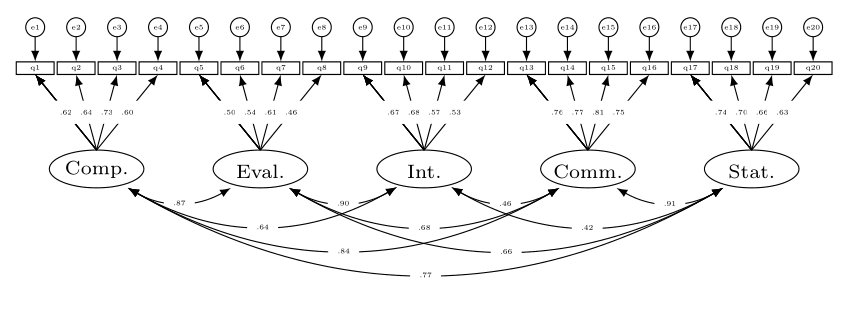
\includegraphics[width=1.2\textwidth]{images/Model5.png}
    }
    \small 
    \textit{Note.} \raggedright This figure displays the configural measurement model of the data literacy items within the training sample, showing standardized factor loadings and latent covariances. The abbreviations q1 up to q20 represent the items, the abbreviations e1 up to e20 their respective residuals. The abbreviations, Comprehension (Comp.), Evaluation (Eval.), Integration (Int.), Communication (Comm.), and Statistics (Stat.) indicate which is the respective latent factor.
\end{figure}
\vspace{0.3cm}

For the configural model of the training sample in the MGCFA, standardized loadings of the factor Comprehension ranged from .58 to .77. For the factor Evaluation loadings ranged from .35 to .74. For the factor Integration loadings ranged from .46 to .78. For the factor Communication loadings ranged from .56 to .75. For the factor Statistics loadings ranged from .60 to .74. The complete model is also displayed in Figure 3.

\vspace{0.3cm}
\begin{figure}
    \centering
    \caption{Measurement Model of the MGCFA Model in the test sample.} 
    \makebox[\textwidth][c]{%
        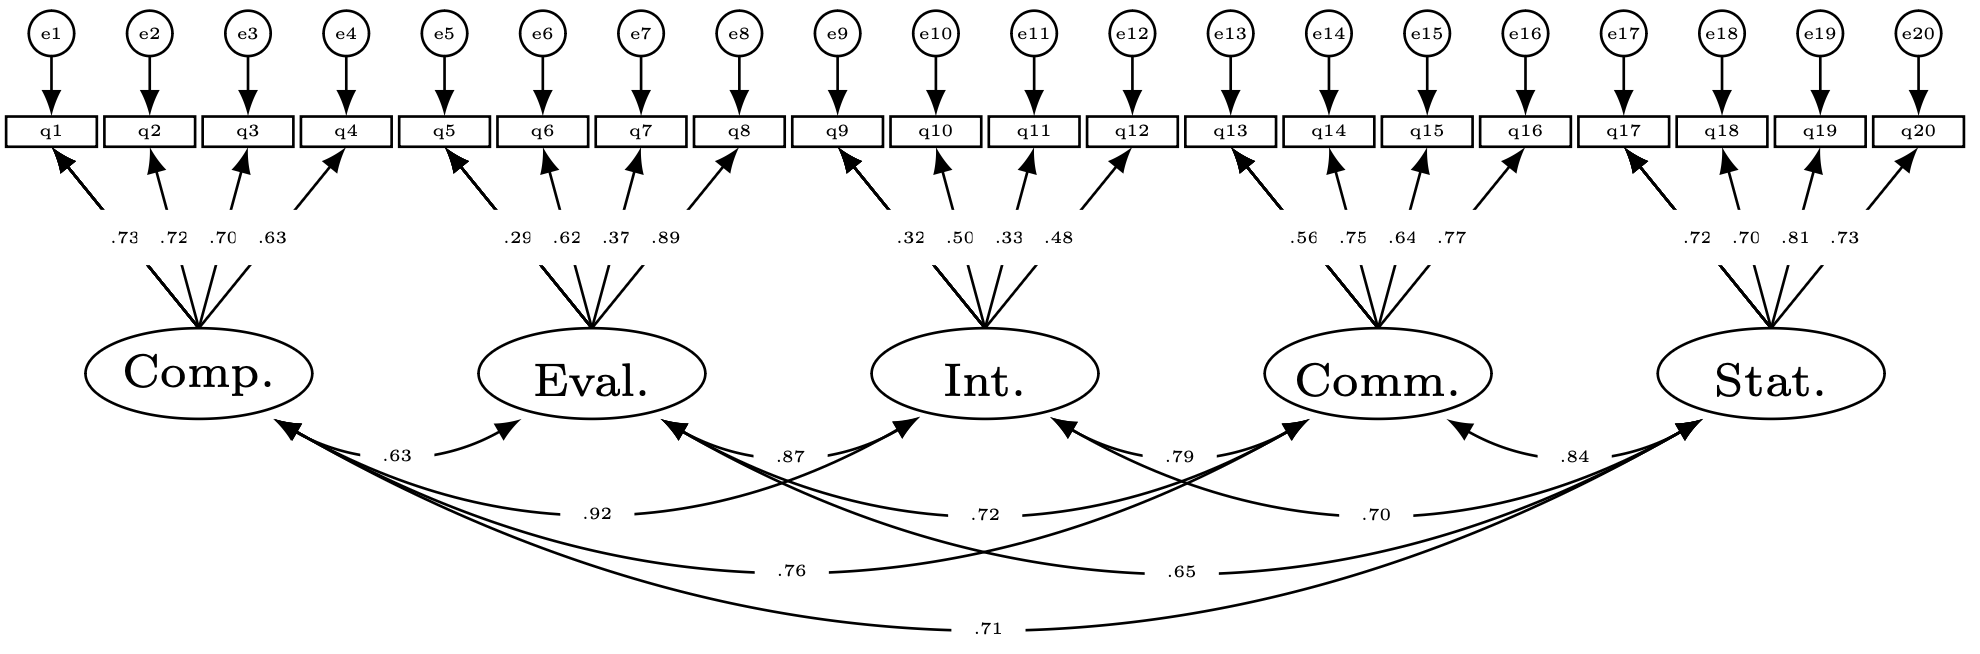
\includegraphics[width=1.2\textwidth]{images/Model6.png}
    }
    \small
    \textit{Note.} \raggedright This figure displays the configural measurement model of the data literacy items within the test sample, showing standardized factor loadings and latent covariances. The abbreviations q1 up to q20 represent the items, the abbreviations e1 up to e20 their respective residuals. The abbreviations, Comprehension (Comp.), Evaluation (Eval.), Integration (Int.), Communication (Comm.), and Statistics (Stat.) indicate which is the respective latent factor.
\end{figure}
\vspace{0.3cm}

For the configural model of the test sample in the MGCFA, standardized loadings of the factor Comprehension ranged from .63 to .73. For the factor Evaluation loadings ranged from .29 to .89. For the factor Integration loadings ranged from .32 to .77. For the factor Communication loadings ranged from .56 to .77. For the factor Statistics loadings ranged from .70 to .81. The complete model is also displayed in Figure 4.
Cross-validation of the MGCFA with the test-data indicated that the assumption of scalar invariance holds across the two subsamples: \(X^{2}\)(\emph{df} = 389) = 659.746, \(p\) \textless{} 0.001, CFI = .92, SRMR = .087, RMSEA = .038; \(\Delta\text{CFI}\) \textless{} .00 , \(\Delta\text{SRMR}\) \textless{} .00, \(\Delta\text{RMSEA}\) = .001 (cf.~Table 2). This indicates support for the second hypothesis (H2).

\begin{table}[htpb]
\caption{Fit Indices for Model and Results of MGCFA testing}
\resizebox{\textwidth}{!}{
\small
\begin{tabular}{cccccccc}
\hline
Model &  Invariance level & CFI & RMSEA & SRMR & $\Delta$ CFI & $\Delta$ RMSEA & $\Delta$ SRMR \\
\hline
 Model 1 & Configural  &  .92 & .041 & .086 & - & - & -\\
  & Metric   &  .92 & .039 & .087 & .002 & .002 & .001\\
  & Scalar   & .92 & .038 & .087 & - & .001 & - \\
  & Residual & .91 & .041 & .092 & \textbf{.015} & .003 & .005\\
 
\hline
\end{tabular}
}

\vspace{10pt}
\small\textit{Note}. The table shows the essential fit indices of the model created with 'stuart', alongside their change in terms of Invariance testing, per invariance level. All Indices shown were estimated with ML as estimator.
\end{table}

The model of the final set of items shows McDonald's \(\omega\)\textsubscript{total} = .92. The composite values McDonald's \(\omega\)\textsubscript{total} of the factors are Comprehension = .76, Evaluation = .65, Integration = .67, Communication = .81 and Statistics = .68.
While overall fit indices (e.g., RMSEA, CFI) suggest a good fit, an analysis of correlated residual was done to reveal possible specification errors.
The correlated residuals from the training sample as well as from the testing sample, can be seen in the appendix (cf.~Table A2 \& Table A3).
Both samples show several residuals to be correlated.

\begin{table}[htpb]
\caption{Latent Factor correlations training sample}

\resizebox{\textwidth}{!}{  
\begin{tabular}{lccccc}
\hline
& Comprehension & Evaluation & Integration & Communication & Statistics \\
\hline
Comprehension & 1.000 & & & & \\
Evaluation    & 0.672 & 1.000 & & & \\
Integration   & 0.596 & 0.715 & 1.000 & & \\
Communication & 0.735 & 0.720 & 0.604 & 1.000 & \\
Statistics    & 0.782 & 0.649 & 0.700 & \textbf{0.971} & 1.000 \\
\hline
\end{tabular}
}

\vspace{10pt}  % Adjust space between table and note
\small\textit{Note}. The table shows the correlations between the latent factors for the training sample.
\end{table}

\subsection{Multicollinearity}\label{multicollinearity}

To furthermore investigate the model, the covariances of the latent factors were examined. The factor correlations for the training sample are displayed in Table 2. The correlation of .97 between Communication and Statistics is to be highlighted. The correlations for the test sample are displayed in Table 3. In the test sample the correlation of .84 between Communication and Statistics is to be highlighted, alongside the correlation of .92 between Comprehension and Integration, as well as the correlation of .87 between Evaluation and Integration. Especially the correlations, that exceed .90 suggest multicollinearity in the data.

\begin{table}[htpb]
\caption{Latent Factor correlations test sample}

\resizebox{\textwidth}{!}{ 
\begin{tabular}{lccccc}
\hline
& Comprehension & Evaluation & Integration & Communication & Statistics \\
\hline
Comprehension & 1.000 & & & & \\
Evaluation    & 0.627 & 1.000 & & & \\
Integration   & \textbf{0.918} & \textbf{0.870} & 1.000 & & \\
Communication & 0.760 & 0.432 & 0.799 & 1.000 & \\
Statistics    & 0.707 & 0.361 & 0.694 & \textbf{0.837} & 1.000 \\
\hline
\end{tabular}
}

\vspace{10pt}  % Adjust space between table and note
\small\textit{Note}. The table shows the correlations between the latent factors for the test sample.
\end{table}

\subsection{Criterion Validity}\label{criterion-validity}

For the correlations, Kendall's rank correlation coefficient (\(\tau\)) was estimated, because the data was not normally distributed. The factors (Comprehension, Evaluation, Integration, Communication \& Statistics) of the data literacy scale correlated moderately to highly with the SWE-IV-16 ( \(\tau\) =.47, \(\tau\) =.46, \(\tau\) =.40, \(\tau\) =.48, \(\tau\) =.39 ; all \(p\) \textless{} .01). The factors of data literacy showed small to moderate correlations with the NFC-K (\(\tau\) =.22, \(\tau\) =.24, \(\tau\) =.30, \(\tau\) =.37, \(\tau\) =.42; all \(p\) \textless{} .01). The factors of the data literacy scale showed moderate correlations with the general items of the ICT-SC25 (\(\tau\) =.31, \(\tau\) =.17, \(\tau\) =.23, \(\tau\) =.43, \(\tau\) =.32; all \(p\) \textless{} .01). The factors Comprehension, Evaluation and Integration correlated slightly negative with the openness of the BFI-10 (\(\tau\) = -.15, \(p\) \textless{} .05; \(\tau\) = -.18, \(p\) \textless{} .01; \(\tau\) = -.26, \(p\) \textless{} .01). Openness did not correlate statistically significant with the other factors. The factors Comprehension, Evaluation, Communication and Statistics correlated slightly up to moderate with conscientiousness of the BFI-10 (\(\tau\) = .13, \(p\) \textless{} .05; \(\tau\) = .25, \(p\) \textless{} .01; \(\tau\) = .16, \(p\) \textless{} .05; \(\tau\) = .17, \(p\) \textless{} .01). The latent correlations with respective confidence intervals are also displayed in table 6.
Those results indicate support for the hypotheses 3, 4 and 7 (H3, H4 \& H7), while not supporting the hypotheses 5 and 6 (H5 \& H6).

\begin{table}[htbp]
\centering
\rotatebox{90}{ %
\begin{minipage}{\textheight} % Ensures caption is properly associated with the rotated content
\caption{Means with standard deviations, and correlations with confidence intervals}
\small
\begin{tabular}{lccccccccccc}
\hline
\textbf{Var} & \textit{M} & \textbf{1} & \textbf{2} & \textbf{3} & \textbf{4} & \textbf{5} & \textbf{6} & \textbf{7} & \textbf{8} & \textbf{9} \\
\hline
1. Con. & 3.68 & & & & & & & & & \\
   & [0.76] & & & & & & & & & \\
2. Open & 2.18 & -0.09 & & & & & & & & \\
   & [0.87] & [-0.21, 0.04] & & & & & & & & \\
3. Nfc & 4.89 & 0.16* & -0.06 & & & & & & & \\
   & [1.07] & [0.04, 0.28] & [-0.19, 0.06] & & & & & & & \\
4. Ict & 4.03 & 0.03 & -0.04 & 0.18** & & & & & & \\
   & [0.72] & [-0.10, 0.16] & [-0.16, 0.09] & [0.06, 0.30] & & & & & & \\
5. Swe & 3.66 & 0.38** & -0.24** & 0.30** & 0.34** & & & & & \\
   & [0.53] & [0.26, 0.48] & [-0.36, -0.12] & [0.19, 0.41] & [0.23, 0.45] & & & & & \\
6. Comp. & -0.03 & 0.13* & -0.15* & 0.22** & 0.31** & 0.47** & & & & \\
   & [0.85] & [0.01, 0.26] & [-0.28, -0.03] & [0.10, 0.34] & [0.19, 0.43] & [0.37, 0.56] & & & & \\
7. Eval. & -0.00 & 0.25** & -0.18** & 0.24** & 0.17** & 0.46** & 0.32** & & & \\
   & [0.54] & [0.12, 0.36] & [-0.30, -0.05] & [0.12, 0.36] & [0.04, 0.29] & [0.35, 0.55] & [0.20, 0.43] & & & \\
8. Int. & -0.01 & 0.05 & -0.26** & 0.30** & 0.23** & 0.40** & 0.28** & 0.26** & \\
   & [0.54] & [-0.07, 0.18] & [-0.37, -0.14] & [0.18, 0.41] & [0.11, 0.35] & [0.28, 0.50] & [0.16, 0.40] & [0.13, 0.37] & \\
9. Comm. & 0.01 & 0.16* & -0.10 & 0.37** & 0.43** & 0.48** & 0.52** & 0.27** & 0.34** \\
   & [0.92] & [0.04, 0.28] & [-0.23, 0.02] & [0.26, 0.48] & [0.33, 0.53] & [0.37, 0.57] & [0.42, 0.61] & [0.15, 0.38] & [0.22, 0.45] \\
10. Stat. & 0.03 & 0.17** & -0.04 & 0.42** & 0.32** & 0.39** & 0.40** & 0.18** & .30** & 0.61** \\
   & [1.00] & [0.04, 0.29] & [-0.17, 0.09] & [0.30, 0.52] & [0.20, 0.43] & [0.27, 0.49] & [0.29, 0.51] & [0.05, 0.30]& [0.18, 0.41 ] & [0.53, 0.69] \\
\hline
\end{tabular}
\par % Ensures separation of the table and note
\small\textit{Note}. The table displays values of Kendalls tau. \textit{M} and \textit{SD} are used to represent mean and standard deviation, respectively. Values in square brackets beneath the M show the respective standard deviation. The other values in square brackets indicate the 95\% confidence interval for each correlation. The confidence interval is a plausible range of population correlations that could have caused the sample correlation (Cumming, 2014). * indicates $p < .05$. ** indicates $p < .01$.
\end{minipage}%
}
\end{table}

\subsection{Control Variables}\label{control-variables}

The analysis of control variables (gender, educational level, aspired degree, and occupation classification) revealed that most items showed no statistically significant effects. Singularity issues, particularly in degree and occupation categories, further limited the interpretability of some results.\\
For `Education 5' (A-levels), a statistically significant negative effect was found on F2F15 (\(b\) = -3.00, \(p\) = 0.03), indicating an average score 3.0 points lower than individuals within the reference group. Conversely, A-levels had a positive effect on F4F3 (\(b\) = 3.91, \(p\) = 0.04). Education also influenced F4F8, where A-levels (\(b\) = 2.82, \(p\) = 0.02), `Education 7' (degree from a university of applied sciences) (\(b\) = 7.46, \(p\) = 0.00), and `Education 8' (university degree) (\(b\) = 7.04, \(p\) = 0.00) also showed statistically significant positive effects.\\
`Degree 2' (Masters) showed a statistically significant negative effect on F4F8 (\(b\) = -3.20, \(p\) = 0.05), while `Degree 3' (state examination) had a positive effect (\(b\) = 2.60, \(p\) = 0.03). On F5F8, pursuing a state examination showed a positive effect (\(b\) = 3.00, \(p\) = 0.05), while pursuing a Master and `Degree 4' (doctorate) encountered singularity issues and could not be estimated.\\
Finally, for `Age 22', a statistically significant negative effect was found on F5F8 (\(b\) = -3.00, \(p\) \textless{} 0.05), indicating individuals aged 22 scored, on average, 3.00 points lower than the reference group.

\section{Discussion}\label{discussion}

This study meant to examine whether 20 items out of the initial item pool, would reflect the suggested measurement model within the current sample. Furthermore, the aim was to find a solution utilizing the genetic algorithm as well as a 3-fold crossvalidation in `stuart', that yields good model fit as well as reliability, and that shows measurement invariance with a random split-sample. Additionally, correlations with other scales and constructs were to be examined to locate the construct within the nomological net.
The model demonstrating the best overall fit was selected, based on a set of 20 items representing five factors: Comprehension, Evaluation, Integration, Communication, and Statistics, each with four items and respective measurement errors. The model also included inter-factor correlations between all latent factors.
Construct validity was evaluated through CFA, using MLR as estimator, as well as correlation analyses with related constructs.

\subsection{Model fit Initial Item Selection}\label{model-fit-initial-item-selection}

Although the RMSEA was a bit low, the initial model exhibited an acceptable to good fit, with indices suggesting good model fit (RMSEA = 0.05, SRMR = 0.08, CFI = 0.96), according to Hu \& Bentler (\citeproc{ref-hu1999}{1999}).
However, recent advancements in scientific methods, such as the ``ezCutoffs'' package (\citeproc{ref-schmalbach2019}{Schmalbach et al., 2019}), propose simulated cutoffs that adapt to specific model characteristics, potentially offering a more rigorous and context-sensitive approach to assessing model fit.
According to this, the following cutoffs are suggested: scaled CFI: .986; scaled RMSEA: .022 and SRMR: .041.
Respectively, the model exhibits non-acceptable fit.
It is argued, that fixed cutoffs are derived from specific confirmatory factor analysis models and may not perform well under varying conditions, such as sample size, model complexity, and response types (\citeproc{ref-Goretzko2023}{Goretzko et al., 2023}; \citeproc{ref-mcneish_wolf_2023}{McNeish \& Wolf, 2023}).
This woult suggests that while traditional cutoffs provide a useful starting point, they may not adequately capture the nuances of different modeling scenarios.
The factor loadings ranged from 0.50 to 0.81 across the five factors (cf.~Figure 1), and the models McDonald's \(\omega\)\textsubscript{total} was 0.92, indicating reliable internal consistency.
Regarding the first hypothesis (H1) it can be concluded, that the algorithm was able to find a solution, exhibiting good model fit according to Hu \& Bentler (\citeproc{ref-hu1999}{1999}), in the training sample, for the suggested measurement model.
However, according to the cutoffs from the ``ezCutoffs'' package (\citeproc{ref-schmalbach2019}{Schmalbach et al., 2019}), the H1 would not be supported.

\subsection{Measurement Invariance and Model Fit}\label{measurement-invariance-and-model-fit}

For further validation, the model was tested for measurement invariance against the test-sample.
The results suggests that invariance levels up to scalar invariance hold (cf.~Table 3).
This conclusion is drawn based on the fit indices remaining within the acceptable range proposed by F. F. Chen (\citeproc{ref-chen2007}{2007}).
However, given that fit indices are regarded more as rough guidelines than as precise or universally applicable cut-off values, an additional perspective was considered.
Specifically, the differences between the (robust) confirmatory fit indices were examined to ensure they remained below 0.01, as recommended by Cheung \& Rensvold (\citeproc{ref-cheung2002}{2002}).\\
In practical terms, when scalar invariance holds, the factor loadings, intercepts, and measurement scales can be considered equivalent across groups.
Thus, the data indicates that all factor loadings are consistent across groups (\citeproc{ref-cheung2002}{Cheung \& Rensvold, 2002}).
This suggests that the data literacy items and their underlying factors are associated with the same strengths in both samples. Additionally, scalar invariance was established, implying that beyond the factorial structure and factor loadings, the item intercepts are also invariant across groups.
This allows for meaningful comparisons of latent means between groups rather than observed differences being due to measurement bias or differences in how the construct is understood or measured across groups (\citeproc{ref-cheung2002}{Cheung \& Rensvold, 2002}; \citeproc{ref-riordan1994}{Riordan \& Vandenberg, 1994}).
The lack of residual invariance suggests that the residuals (unexplained variance in the indicators) are not equivalent across groups. This implies that there are group-specific differences in how much of the variance in the observed variables remains unexplained by the latent factors. Thus, this lack of residual invariance complicates the interpretation of differences between groups (\citeproc{ref-cheung2002}{Cheung \& Rensvold, 2002}). While the factors themselves may be measured similarly (because scalar invariance holds), the amount of unexplained variability in the responses differs across groups, indicating potential unmodeled differences in how the groups respond to certain items.
As a result, any observed differences in the latent factors could be influenced by differing error variances across groups, making it challenging to draw definitive conclusions about true group differences. Thus, while latent means can be compared, the comparisons may be confounded by measurement error that varies across groups.\\
Regarding the second hypothesis (H2) it can be concluded that the latent factor structure of the initial analysis was supported by the test-sample.
It is also to be noted that the model fit on the configural level (RMSEA = 0.041, SRMR = 0.09, CFI = 0.92), according to Hu \& Bentler (\citeproc{ref-hu1999}{1999}) and the `ezCutoffs' package (\citeproc{ref-schmalbach2019}{Schmalbach et al., 2019}), is worse than the fit of the training sample, except for the RMSEA (cf.~Table 3).
The changing of the fit of the test sample is also reflected in the measurement model (cf.~Figure 2).
There does not appear to be a consistent direction of change, as some factor loadings on the items increase while others decrease.
The same applies to the latent correlations between the factors, which could be interpreted as an indication of the solution's instability.

Across the versions of this model, the CFI decreases the most and the RMSEA suffers the least.
As the CFI is comparing the tested models against a base-line model, it could be that the strong decrease in this index reflects the divergence of the model respective to the differing sample and thus indicates overfitting.
Furthermore, some items showed high correlations (cf.~Appendix Table A4), as well as high residual correlations (cf.~Appendix Tables A2 \& A3) (shared variance not explained by the latent factor).
Those correlated residuals, could indicate potential specification errors, both in the training and test sample, therefore the model fit could deteriorate and reduce the CFI.
Furthermore, the latent correlations among factors were overall strong, especially between Communication and Statistics (0.91 in the training sample and 0.84 in the test sample) (cf.~Tables 4 \& 5).
This could indicate redundancy among the factors, that needs to be addressed in terms of items and factor specification.
The SRMR showed mediocre fit, but degrades in the MGCFA and progressively so with increasing the invariance levels. This could in part be due to the fact, that the SRMR makes no correction for parsimony, thus improves the more paths a model contains.
As invariance is increased and paths are constrained to equality, it could make sense for the SRMR to increase.
The RMSEA in turn accounts for some complexity of the model, and also performs better in this case as the SRMR.

\subsection{Construct Validity}\label{construct-validity}

The moderate to high correlations between the newly created data literacy scale and the SWE-IV-16, and the general items of the ICT-SC25 (cf.~Table 6) suggest that the scale measures a concept that is related but distinct.
This supports the expectations outlined in H3 and H4.
The results consistent with H3 and H4, which concern the alignment of the measured latent factors with competency-based constructs, further support the interpretation that the scale captures perceived competency rather than a stable personal character trait.
Those correlations could indicate convergent validity (\citeproc{ref-gregory2004}{Gregory, 2004}).\\
The strong correlation between the data literacy scale and NFC-K are not in line with H5 (cf.~Table 6).
This might reflect conceptual proximity between the two measures, and could indicate that the data literacy questionnaire measures a construct more aligned with trait characteristics than planned.
It is plausible that individuals who enjoy understanding concepts in detail (as measured by NFC-K) also display behaviors associated with critically examining data and information. This finding underscores the relevance of motivation as a contributing factor to the observed behaviors, suggesting conceptual overlapping elements between data literacy and NFC.\\
The data literacy factors also showed small to moderate correlations with personality traits, including a negative correlation with openness and a positive correlation with conscientiousness. The positive association with conscientiousness aligns with H7, indicating that individuals who are organized and diligent may also exhibit behaviors related to data literacy.
This correlation could be an indicator for discriminant validity (\citeproc{ref-cronbach1955}{Cronbach \& Meehl, 1955}; \citeproc{ref-hubley1996}{Hubley \& Zumbo, 1996}).\\
However, the negative correlation with openness contradicts expectations (H6).
Given the conceptualization of data literacy as a proficiency that incorporates motivation to engage in related behaviors, a slight positive correlation with openness was anticipated, as openness typically reflects curiosity and a willingness to explore new ideas, or a persons motivation to show certain behaviors.
The opposite was found.
This unexpected negative relationship could suggest that the items of the data literacy scale emphasize ability or skill over proficiency, thereby capturing behaviors less influenced by intrinsic motivation.\\
Another plausible explanation for the findings would be a mismatch between the items and the study sample. Motivation can be linked to expertise (\citeproc{ref-earley1990}{Earley et al., 1990}; \citeproc{ref-paletz2013}{Paletz et al., 2013}), and participants may perceive the assessed behaviors as routine rather than requiring deliberate effort or motivation. For these individuals, data literacy behaviors might represent habitual actions rather than aspirational or exploratory tendencies.

Paletz et al. (\citeproc{ref-paletz2013}{2013}) highlight that individuals engaged in routine behaviors can identify problems and adapt their processes as they gain experience. This suggests that, as expertise develops, individuals may rely more on established routines rather than on motivation to initiate behaviors. Similarly, Jong \& Fodor (\citeproc{ref-fodor2017}{2017}) suggest that with increased familiarity, task-related behaviors may become less influenced by external motivational factors and instead governed by ingrained, automated routines.
The development of expertise also frequently leads to cognitive simplification of complex tasks. As individuals gain familiarity, they tend to schematize their behaviors into automatic processes, reducing the reliance on deliberate motivational triggers (\citeproc{ref-earley1990}{Earley et al., 1990}). This cognitive simplification allows individuals to focus less on initiating behaviors and more on refining and adapting their routines as needed.\\
Taken together, these perspectives suggest that the role of motivation in data literacy behaviors may diminish with increasing expertise, as participants shift toward automated and habitual patterns of engagement.

\subsection{Control Variables}\label{control-variables-1}

The control variable analysis revealed statistically significant effects of educational level, degree pursuit, and age on specific items. These findings could help to explain how individual characteristics influence self-reported behaviors and competencies and offer insights for educational interventions.
The negative effect of A-levels on F2F15 (``I check the qualifications of authors before relying on the information.'') suggests that individuals with A-levels as their highest educational attainment are less inclined to evaluate an author's qualifications before trusting their information. This may reflect insufficient emphasis on critical evaluation skills at the A-level stage, which are typically developed more extensively in tertiary education. This observation underscores a potential gap in curricula, which could be addressed by integrating critical appraisal training earlier in the educational trajectory. Notably, some German schools have already reformed their curricula to emphasize media competency (\citeproc{ref-mediaeducationlab2020}{Media Education Lab, 2020}; \citeproc{ref-richter_scheiter_2023}{Richter \& Scheiter, 2023}), potentially serving as a model for broader implementation.

For F3F2 (``I deal with information that challenges my views.''), the analysis was inconclusive. Singularities in the data, likely caused by collinearity or insufficient variability in the predictor variables, limit interpretability. This finding highlights a methodological limitation, suggesting that the item F3F2 may lack robustness for statistical modeling in its current form. Future studies should consider refining or reformulating this item to enhance its validity.

A-levels exhibited a positive effect on F4F3 (``I can present data in graphics in such a way that they are understandable for different target groups.''), indicating that A-level graduates report confidence in presenting data graphically to diverse audiences. This may reflect the inclusion of basic communication and data visualization skills in the A-level curriculum, underscoring the value of these foundational competencies at this stage of education.

The results for F4F8 (``I can use programs to create graphics to present results.'') demonstrate a progressive relationship between educational attainment and proficiency with data visualization software. While A-levels are associated with a modest increase (+2.82 points), higher educational levels such as a degree of a university of applied sciences, and a university degree, show substantially larger effects (+7.46 and +7.04 points, respectively). These results likely reflect the greater exposure to specialized tools and training in higher education. Intriguingly, currently pursuing a Master's degree was associated with a negative effect on F4F8 (-3.20 points), potentially indicating transitional challenges or curricular variability in graduate programs. In contrast, currently pursuing a state examination showed a positive effect (+2.60 points), suggesting that this pathway may place greater emphasis on developing these skills.

For F5F8 (``When I am confronted with extensive data sets, I can gain insights from them.''), a statistically significant negative effect was observed for `Age22' (-3.00 points), indicating lower self-reported confidence in extracting insights from large datasets among this age group. This result may reflect developmental factors, such as limited experience or confidence, or contextual influences unique to this stage. However, as no other items showed age-related effects, this finding should be interpreted cautiously. Additionally, while no significant educational variables were identified for F5F8, having a state examination as highest education, demonstrated a significant positive effect (+3.00 points). However, the absence of other degree categories makes a comparison impossible, warranting further investigation.

\subsection{Limitations}\label{limitations}

The results of this study should be interpreted with several limitations in mind. The sample deviates from the general population in multiple demographic variables, potentially compromising its representativeness and generalizability. Occupational distribution among participants shows clustering in fields such as ``Gesundheit, Soziales, Lehre und Erziehung'', ``Buchhaltung, Recht und Verwaltung'', ``Kaufmännische Dienstleistungen, Vertrieb, Tourismus'' and especially ``Naturwissenschaft, Geografie und Informatik''. This indicates a selection bias, likely due to recruitment methods (who is reached) and implicitly favoring individuals more interested in data literacy.

The item pool for the questionnaire was specifically trained on this non-representative sample, which will likely affect its validity.
Because it could result in the creation and measurement of a latent construct that is specific or unique even to this particular sample.
Ideally, this approach would have been used with a sample representative of the general public or citizens.
That way the results would be more valid and could more likely be generalized.
A more representative sample might enhance the indicated effects, making them become clearer.

The visual analysis of item boxplots revealed several outliers in the data. These outliers were retained in the sample for further investigation, as their clustering in the higher categories (4 and 5) suggests that the items may have been too easy for most respondents, resulting in high levels of agreement. This concentration of responses at the upper end of the scale indicates potential ceiling effects, where the items fail to adequately discriminate across a range of respondent abilities. Conversely, the outliers in the lower categories (0, 1, or 2) are relatively rare and unlikely to significantly influence the overall conclusions. However, their presence suggests that a small subset of participants either found the items unclear or disagreed with them, potentially pointing to systematic factors.
The measure was designed with a general population in mind, which may have limited its ability to differentiate at higher levels of item difficulty, particularly among more data-literate participants. Addressing this limitation in future studies would improve the instrument's sensitivity to varying levels of data literacy.
Also, as data literacy is a heterogeneous construct, this complicates global instrument development and understanding across all participants. Ideally the questionnaire would incorporate a broader content to better reflect the constructs full scope, thereby increasing content validity.
However, a broader tool should be designed to maintain sufficient power to detect indicated factor-specific effects.
Expanding the questionnaire with additional items could address this need, although it would deviate from the principle of parsimony.

These issues regarding the misfit of items and sample, as well as the heterogeneity of the construct further result in limitations regarding the reliability of the instrument. Although the McDonald's \(\omega\)\textsubscript{total} would indicate good reliability, the question of reliability stretches beyond a single measure for internal consistency.
The reliability of a measure must be evaluated in relation to its target audience, as its validity and generalizability depend on how well the sample reflects the intended population.
Therefore, it is crucial to determine which sample the measure is based on and the population it aims to represent.

In discussing the characteristics and demographics of the sample, the randomization of the data literacy items among respondents also introduced certain limitations.
The primary limitation lies in the unequal demographic distribution across items.
For example, while the overall sample has an average age of 40 years, this demographic balance may not hold for each individual item.
This issue extends to other demographic variables as well, resulting in the diversity of the sample not being consistently reflected in the responses to individual items.
Consequently, the selected items would require further and coherent testing of the item set as a whole on a diverse sample to evaluate how demographic variability influences responses.
The limited demographic balance in the items also results in limited control for confounding variables in those variables. It furthermore limits the informative value of comparisons regarding the demographic variables among the items.

Additionally, the training and testing data sets differed in size, which could influence measurement invariance testing (\citeproc{ref-chen2007}{F. F. Chen, 2007}). While the sample sizes were appropriate, they were at the lower threshold of the prior power analysis (\citeproc{ref-hu1999}{Hu \& Bentler, 1999}; e.g., \citeproc{ref-kass1979}{Kass \& Tinsley, 1979}), suggesting that larger samples might have been better. Also the 3-folding was on the lower threshold of power with the used sample size and possibly, a larger number of folds could have helped to increase the stability of the solution. Lastly, it should be noted that algorithm-based item selection is a heuristic approach, rather than deterministic, and may not always yield the optimal solution (\citeproc{ref-blum2003}{Blum \& Roli, 2003}; \citeproc{ref-schultze2017}{Schultze, 2017}).
In this specific study, the results of the algorithm based selection with the genetic algorithm in `stuart' appeared to be unstable across different runs.
I tried to account for that via the \(k\)-folding and multiple iterations of the selection, but when the process of the data imputation was changed, from `mice' to FIML, different items were selected, indicating unstable selections.
This could potentially be accounted for, by using the bruteforce implementation in `stuart'.
But it could also be a hint at model misspecification, because of which the algorithm finds multiple local minima.\\
The models yielded rather bad fit measures, when using the initially planned objective function (with the aim of optimising for model fit, reliability, and variability in the difficulty of items.
Therefore, it was changed in favor of model fit criteria exclusively.
Thus, the final objective function that was used, did not incorporate terms to optimize for reliability McDonald's \(\omega\) nor variability in the difficulty of items.\\
Furthermore WLSMV could not be used, although being the appropriate estimator for rating scales, because of the ceiling effects in the items and the scarcely used lower answer categories.
I tried to account for that by collapsing the respective answer categories, but this seemingly resulted in an introduction of better fit to the model. Because of that, I decided to use MLR as estimator and were therefore able to use FIML as imputation method, implemented in `lavaan'.
Ideally future studies, with a sample without ceiling effects, would use WLSMV as estimator, since modified weighted least square estimators for ordered-categorical indicators (MWLS\textsubscript{C}) provide accurate estimates of the model parameters given a stable weight matrix (\citeproc{ref-wirth2007}{Wirth \& Edwards, 2007}) and furthermore, WLSMV is a robust estimator which does not assume normally distributed variables and provides the best option for modelling categorical or ordered data (\citeproc{ref-brown2006}{T. A. Brown, 2006}).

\subsection{Future directions}\label{future-directions}

Future research in this domain should focus on expanding the qualitative development of items to ensure comprehensive coverage of the various dimensions of data literacy. A more extensive qualitative item creation process, informed by interviews with a diverse group of individuals, would contribute to a more nuanced understanding of the construct, particularly across different occupations as well as educational levels. Such qualitative insights could help identify representative behaviors and cognitive processes, forming a more solid foundation for item development. Additionally, these insights would contribute to the establishment of a more robust theoretical model for self-perceived data literacy. Expert interviews would be particularly valuable, integrating multiple perspectives on the construct and providing a more grounded theoretical base.

Future studies should consider assessing whether items in data literacy scales are sensitive to the distinction between routine and aspirational behaviors. Additionally, capturing the progression from motivated to routine actions could provide deeper insights into how expertise shapes self-perceived data literacy.
These findings invite further refinement of the scale to better balance the measurement of skills, proficiencies, and the motivational aspects of data literacy.
Future research should also consider whether the scale captures routine versus intentional behaviors, as this distinction may vary across samples and contexts.

This study clearly highlights that both the measurement model and the items of the scale require revision. Given that data literacy is a heterogeneous and multi-faceted construct, future research should rigorously explore the dimensionality of the scale to ensure its accuracy and utility. A thorough investigation of this dimensionality is essential for the validity of any future attempts at scale validation.
A careful and thorough development of items is necessary to address the multi-faceted nature of the construct. This is particularly important for adapting the scale to measure individual skill levels accurately, which could be achieved through methods such as Item Response Theory (IRT). An IRT-based framework could significantly enhance the scale's precision by allowing for variability in item difficulty, thereby improving the adaptability and accuracy of the measurement. The introduction of adaptive testing, based on IRT principles, could lead to a more efficient scale, requiring fewer items while maintaining or even improving measurement precision.

\subsection{Conclusion}\label{conclusion}

The present study represents a first step towards addressing the gap in tools for measuring self-rated data literacy among the general public.
The final instrument demonstrated acceptable psychometric properties that could be approved upon, including strong internal consistency and promising criterion validity.
While the results validate the scale's potential utility, challenges remain, particularly concerning multicollinearity among producer facets and limitations in the broader generalizability due to sample-specific characteristics. These issues necessitate further refinement of the scale and the respective measurement model. Replication studies would be necessary to establish its reliability and invariance across diverse populations. Future research should also explore the practical implications of enhancing data literacy in educational and societal frameworks, addressing the critical role of such competencies in an increasingly data-driven world.
In conclusion, this thesis provides a foundational contribution to the emerging field of data literacy research. It lays a solid groundwork for future studies, emphasizing the need for ongoing refinement and broader validation efforts to fully realize the scale's potential in fostering data-literate societies.

\section*{References}\label{references}
\addcontentsline{toc}{section}{References}

\phantomsection\label{refs}
\begin{CSLReferences}{1}{0}
\bibitem[\citeproctext]{ref-algner2022}
Algner, M., \& Lorenz, T. (2022). You're prettier when you smile: Construction and validation of a questionnaire to assess microaggressions against women in the workplace. \emph{Frontiers in Psychology}, \emph{13}. \url{https://doi.org/10.3389/fpsyg.2022.809862}

\bibitem[\citeproctext]{ref-ACRL2000}
Association of College \& Research Libraries. (2000). \emph{Information literacy competency standards for higher education}. Brochure; American Library Association.

\bibitem[\citeproctext]{ref-Bartholomew2009}
Bartholomew, D. J., Deary, I. J., \& Lawn, M. (2009). The origin of factor scores: Spearman, thomson and bartlett. \emph{British Journal of Mathematical and Statistical Psychology}, \emph{62}, 569--582. \url{https://doi.org/10.1348/000711008x365676}

\bibitem[\citeproctext]{ref-bates2009}
Bates, M. J. (2009). \emph{An introduction to metatheories, theories, and models}. \url{https://api.semanticscholar.org/CorpusID:62396882}

\bibitem[\citeproctext]{ref-behm2018}
Behm, T. (2018). \emph{SWE-IV-16: Skala zur erfassung der informationsverhaltensbezogenen selbstwirksamkeitserwartung {[}verfahrensdokumentation, fragebogen deutsche und englische version (SES-IB-16){]}} {[}Open Test Archive{]}. Leibniz-Institut für Psychologie (ZPID). \url{https://doi.org/10.23668/psycharchives.4598}

\bibitem[\citeproctext]{ref-beiuxdfert2015}
Beißert, H., Köhler, M., Rempel, M., \& Beierlein, C. (2015). Deutschsprachige kurzskala zur messung des konstrukts need for cognition NFC-k. \emph{Zusammenstellung Sozialwissenschaftlicher Items Und Skalen (ZIS)}. \url{https://doi.org/10.6102/zis230}

\bibitem[\citeproctext]{ref-bless1994}
Bless, H., Wänke, M., Bohner, G., Fellhauer, R., \& Schwarz, N. (1994). Need for cognition: Eine skala zur erfassung von engagement und freude bei denkaufgaben {[}presentation and validation of a german version of the need for cognition scale{]}. \emph{Zeitschrift Für Sozialpsychologie}, \emph{25}, 147--154.

\bibitem[\citeproctext]{ref-blum2003}
Blum, C., \& Roli, A. (2003). Metaheuristics in combinatorial optimization: Overview and conceptual comparison. \emph{ACM Comput. Surv.}, \emph{35}(3), 268--308. \url{https://doi.org/10.1145/937503.937505}

\bibitem[\citeproctext]{ref-brandgruwel2009}
Brand-Gruwel, S., Wopereis, I., \& Walraven, A. (2009). A descriptive model of information problem solving while using internet. \emph{Computers \& Education}, \emph{53}(4), 1207--1217. https://doi.org/\url{https://doi.org/10.1016/j.compedu.2009.06.004}

\bibitem[\citeproctext]{ref-brandmaier2024}
Brandmaier, A. M., \& Peikert, A. (2024). Automated reproducibility testing in r markdown. \emph{Preprint}.

\bibitem[\citeproctext]{ref-brillouin1953}
Brillouin, L. (1953). Negentropy principle of information. \emph{Journal of Applied Physics}, \emph{24}(9), 1152--1163.

\bibitem[\citeproctext]{ref-brown2002}
Brown, C., \& Krumholz, L. R. (2002). Integrating information literacy into the science curriculum. \emph{College \& Research Libraries}, \emph{63}, 111--123. \url{https://doi.org/10.5860/crl.63.2.111}

\bibitem[\citeproctext]{ref-brown2006}
Brown, T. A. (2006). \emph{Confirmatory factor analysis for applied research}. Guilford Press.

\bibitem[\citeproctext]{ref-buehner2021}
Bühner, M. (2021). \emph{Einführung in die test- und fragebogenkonstruktion} (4., korrigierte und erweiterte Auflage, p. 752). Hogrefe Verlag.

\bibitem[\citeproctext]{ref-BfA2024}
Bundesargentur für Arbeit. (2024). \emph{Arbeitslosenzahl in deutschland im jahresdurchschnitt von 2005 bis 2024}. \url{https://de.statista.com/statistik/daten/studie/1223/umfrage/arbeitslosenzahl-in-deutschland-jahresdurchschnittswerte/\#:~:text=Im\%20Monat\%20Juni\%202024\%20waren,um\%20rund\%20178.800\%20Personen\%20höher}; Statista.

\bibitem[\citeproctext]{ref-buss1983}
Buss, D., \& Craik, K. (1983). The act frequency approach to personality. \emph{Psychological Review}, \emph{90}, 105--126. \url{https://doi.org/10.1037/0033-295X.90.2.105}

\bibitem[\citeproctext]{ref-cacioppo1982}
Cacioppo, J. T., \& Petty, R. E. (1982). The need for cognition. \emph{Journal of Personality and Social Psychology}, \emph{42}(1), 116--131. \url{https://doi.org/10.1037/0022-3514.42.1.116}

\bibitem[\citeproctext]{ref-callingham2006}
Callingham, R. (2006). Assessing statistical literacy: A question of interpretation? \emph{International Conference on Teaching Statistics (ICOTS7)}.

\bibitem[\citeproctext]{ref-prado2013}
Calzada-Prado, F. J., \& Marzal, M. Á. (2013). Incorporating data literacy into information literacy programs: Core competencies and contents. \emph{Libri}, \emph{63}(2), 123--134. \url{https://doi.org/10.1515/libri-2013-0010}

\bibitem[\citeproctext]{ref-carlson2014}
Carlson, J., Fosmire, M., Miller, C. C., \& Nelson, M. S. (2014). Determining data information literacy needs. In J. Carlson \& M. Johnston (Eds.), \emph{Data information literacy: Librarians, data, and the education of a new generation of researchers}. Purdue University Press.

\bibitem[\citeproctext]{ref-Carmi2020}
Carmi, E., Yates, S. J., Lockley, E., \& Pawluczuk, A. (2020). Data citizenship: Rethinking data literacy in the age of disinformation, misinformation, and malinformation. \emph{Internet Policy Review}, \emph{9}(2). \url{https://doi.org/10.14763/2020.2.1481}

\bibitem[\citeproctext]{ref-carroll1993}
Carroll, J. B. (1993). \emph{Human abilities: Their nature and measurement}. Cambridge University Press.

\bibitem[\citeproctext]{ref-chen2007}
Chen, F. F. (2007). Sensitivity of goodness of fit indexes to lack of measurement invariance. \emph{Structural Equation Modeling: A Multidisciplinary Journal}, \emph{14}(3), 464--504. \url{https://doi.org/10.1080/10705510701301834}

\bibitem[\citeproctext]{ref-Chen2024}
Chen, F., Cui, Y., Lutsyk-King, A., Gao, Y., Liu, X., Cutumisu, M., \& Leighton, J. P. (2024). Validating a novel digital performance-based assessment of data literacy: Psychometric and eye-tracking analyses. \emph{Education and Information Technologies}, \emph{29}(8), 9417--9444. \url{https://doi.org/10.1007/s10639-023-12177-7}

\bibitem[\citeproctext]{ref-cheung2002}
Cheung, G. W., \& Rensvold, R. B. (2002). Evaluating goodness-of-fit indexes for testing measurement invariance. \emph{Structural Equation Modeling: A Multidisciplinary Journal}, \emph{9}(2), 233--255. \url{https://doi.org/10.1207/S15328007SEM0902_5}

\bibitem[\citeproctext]{ref-cohen1955}
Cohen, A. R., Stotland, E., \& Wolfe, D. M. (1955). An experimental investigation of need for cognition. \emph{The Journal of Abnormal and Social Psychology}, \emph{51}(2), 291--294. \url{https://doi.org/10.1037/h0042761}

\bibitem[\citeproctext]{ref-costa1992}
Costa, P. T., \& McCrae, R. R. (1992). The five-factor model of personality and its relevance to personality disorders. \emph{Journal of Personality Disorders}, \emph{6}(4), 343--359. \url{https://doi.org/10.1521/pedi.1992.6.4.343}

\bibitem[\citeproctext]{ref-cronbach1955}
Cronbach, L. J., \& Meehl, P. E. (1955). Construct validity in psychological tests. \emph{Psychological Bulletin}, \emph{52}(4), 281.

\bibitem[\citeproctext]{ref-Cui2023}
Cui, Y., Chen, F., Lutsyk, A., Leighton, J., \& Cutumisu, M. (2023). Data literacy assessments: A systematic literature review. \emph{Assessment in Education: Principles, Policy \& Practice}, \emph{30}, 1--21. \url{https://doi.org/10.1080/0969594X.2023.2182737}

\bibitem[\citeproctext]{ref-deahl2014}
Deahl, E. (2014). \emph{Better the data you know: Developing youth data literacy in schools and informal learning environments} {[}M.S. Thesis{]}. Massachusetts Institute of Technology.

\bibitem[\citeproctext]{ref-dweck1988}
Dweck, C., \& Leggett, E. L. (1988). A social-cognitive approach to motivation and personality. \emph{Psychological Review}, \emph{95}(2), 256--273. \url{https://doi.org/10.1037/0033-295X.95.2.256}

\bibitem[\citeproctext]{ref-earley1990}
Earley, P. C., Lee, C., \& Hanson, L. A. (1990). Joint moderating effects of job experience and task component complexity: Relations among goal setting, task strategies, and performance. \emph{Journal of Organizational Behavior}, \emph{11}(1), 3--15. \url{https://doi.org/10.1002/job.4030110104}

\bibitem[\citeproctext]{ref-elander2004}
Elander, J. (2004). Student assessment from a psychological perspective. \emph{Psychology Learning \& Teaching}, \emph{3}(2), 114--121. \url{https://doi.org/10.2304/plat.2003.3.2.114}

\bibitem[\citeproctext]{ref-fowler1995}
Fowler, Jr., F. J. (1995). \emph{Improving survey questions: Design and evaluation}. Sage Publications, Inc.

\bibitem[\citeproctext]{ref-frank2016}
Frank, M., Walker, J., Attard, J., \& Tygel, A. (2016). Data literacy: What is it and how can we make it happen? editorial. \emph{The Journal of Community Informatics}, \emph{12}(3), 4--8.

\bibitem[\citeproctext]{ref-Gal2002}
Gal, I. (2002). Adults' statistical literacy: Meanings, components, responsibilities. \emph{International Statistical Review / Revue Internationale de Statistique}, \emph{70}(1), 1--25. \url{https://doi.org/10.2307/1403713}

\bibitem[\citeproctext]{ref-galan2013}
Galán, S. F., Mengshoel, O. J., \& Pinter, R. (2013). A novel mating approach for genetic algorithms. \emph{Evolutionary Computation}, \emph{21}(2), 197--229. \url{https://doi.org/10.1162/EVCO_a_00067}

\bibitem[\citeproctext]{ref-Goretzko2023}
Goretzko, D., Siemund, K., \& Sterner, P. (2023). Evaluating model fit of measurement models in confirmatory factor analysis. \emph{Educational and Psychological Measurement}, \emph{84}(1), 123--144. \url{https://doi.org/10.1177/00131644231163813}

\bibitem[\citeproctext]{ref-gould2017}
Gould, R. (2017). Data literacy is statistical literacy. \emph{Statistics Education Research Journal}, \emph{16}(1), 22--25. \url{https://doi.org/10.52041/serj.v16i1.209}

\bibitem[\citeproctext]{ref-green1998}
Green, F. (1998). \emph{The value of skills} (Department of Economics Discussion Paper No. 9819). University of Kent, Department of Economics.

\bibitem[\citeproctext]{ref-gregory2004}
Gregory, R. J. (2004). \emph{Psychological testing: History, principles, and applications}. Pearson Education India.

\bibitem[\citeproctext]{ref-holland1992}
Holland, J. H. (1992). \emph{{Adaptation in Natural and Artificial Systems: An Introductory Analysis with Applications to Biology, Control, and Artificial Intelligence}}. The MIT Press. \url{https://doi.org/10.7551/mitpress/1090.001.0001}

\bibitem[\citeproctext]{ref-hu1999}
Hu, L., \& Bentler, P. M. (1999). Cutoff criteria for fit indexes in covariance structure analysis: Conventional criteria versus new alternatives. \emph{Structural Equation Modeling: A Multidisciplinary Journal}, \emph{6}(1), 1--55. \url{https://doi.org/10.1080/10705519909540118}

\bibitem[\citeproctext]{ref-hubley1996}
Hubley, A. M., \& Zumbo, B. D. (1996). A dialectic on validity: Where we have been and where we are going. \emph{The Journal of General Psychology}, \emph{123}(3), 207--215.

\bibitem[\citeproctext]{ref-jaynes1957}
Jaynes, E. T. (1957). Information theory and statistical mechanics. \emph{Physical Review}, \emph{106}(4), 620--630.

\bibitem[\citeproctext]{ref-john2008}
John, O., Naumann, L., \& Soto, C. (2008). Paradigm shift to the integrative big five trait taxonomy: History, measurement, and conceptual issues. In \emph{Handbook of Personality: Theory and Research, 3rd Edn.} (pp. 114--158).

\bibitem[\citeproctext]{ref-fodor2017}
Jong, J. P. d., \& Fodor, O. C. (2017). Attuning to individual work routines and team performance. \emph{Team Performance Management}, \emph{23}(7/8), 385--406. \url{https://doi.org/10.1108/tpm-01-2017-0001}

\bibitem[\citeproctext]{ref-kass1979}
Kass, R. A., \& Tinsley, H. E. A. (1979). Factor analysis. \emph{Journal of Leisure Research}, \emph{11}(2), 120--138. \url{https://doi.org/10.1080/00222216.1979.11969385}

\bibitem[\citeproctext]{ref-Kendall1938}
Kendall, M. G. (1938). A new measure of rank correlation. \emph{Biometrika}, \emph{30}(1/2), 81--93. \url{http://www.jstor.org/stable/2332226}

\bibitem[\citeproctext]{ref-kerber2022}
Kerber, A., Schultze, M., Müller, S., Rühling, R. M., Wright, A. G. C., Spitzer, C., Krueger, R. F., Knaevelsrud, C., \& Zimmermann, J. (2022). Development of a short and ICD-11 compatible measure for DSM-5 maladaptive personality traits using ant colony optimization algorithms. \emph{Assessment}, \emph{29}(3), 467--487. \url{https://doi.org/10.1177/1073191120971848}

\bibitem[\citeproctext]{ref-keshavarz2021}
Keshavarz, H. (2021). \emph{Personality factors and knowledge sharing behavior in information services: The mediating role of information literacy competencies}. \url{https://doi.org/10.1108/VJIKMS-05-2020-0095}

\bibitem[\citeproctext]{ref-Koltay2017}
Koltay, T. (2017). Information overload in a data-intensive world. In A. J. Schuster (Ed.), \emph{Understanding information: From the big bang to big data} (pp. 197--217). Springer International Publishing. \url{https://doi.org/10.1007/978-3-319-59090-5_10}

\bibitem[\citeproctext]{ref-komarraju2009}
Komarraju, M., Karau, S. J., \& Schmeck, R. R. (2009). Role of the big five personality traits in predicting college students' academic motivation and achievement. \emph{Learning and Individual Differences}, \emph{19}(1), 47--52. \url{https://doi.org/10.1016/j.lindif.2008.07.001}

\bibitem[\citeproctext]{ref-komarraju2011}
Komarraju, M., Karau, S. J., Schmeck, R. R., \& Advic, A. (2011). The big five personality traits, learning styles, and academic achievement. \emph{Personality and Individual Differences}, \emph{51}(4), 472--477. \url{https://doi.org/10.1016/j.paid.2011.04.019}

\bibitem[\citeproctext]{ref-kouts-klemm2019}
Kõuts-Klemm, R. (2019). Data literacy among journalists: A skills-assessment based approach. \emph{Central European Journal of Communication}, \emph{12}(24), 299--315. \url{https://doi.org/10.19195/1899-5101.12.3(24).2}

\bibitem[\citeproctext]{ref-Leighton2021}
Leighton, J. P., Cui, Y., \& Cutumisu, M. (2021). Key information processes for thinking critically in data-rich environments. \emph{Frontiers in Education}, \emph{6}. \url{https://doi.org/10.3389/feduc.2021.561847}

\bibitem[\citeproctext]{ref-leite2008}
Leite, W. L., Huang, I.-C., \& Marcoulides, G. A. (2008). Item selection for the development of short forms of scales using an ant colony optimization algorithm. \emph{Multivariate Behavioral Research}, \emph{43}, 411--431. \url{https://doi.org/10.1080/00273170802285743}

\bibitem[\citeproctext]{ref-lusiyana2020}
Lusiyana, A., Festiyed, F., \& Yulkifli, Y. (2020). Measuring the physics students' data literacy skill in the era of industry 4.0 by using mirecal learning model. \emph{International Journal of Scientific and Technology Research}, \emph{9}(1), 1203--1205. \url{https://api.semanticscholar.org/CorpusID:216552579}

\bibitem[\citeproctext]{ref-mahmood2021}
Mahmood, M., Frolova, Y., \& Gupta, B. (2021). The HEXACO, academic motivation and learning approaches: Evidence from a central asian country. \emph{Education + Training}, \emph{63}(6), 920--938. \url{https://doi.org/10.1108/ET-11-2019-0257}

\bibitem[\citeproctext]{ref-mcneish_wolf_2023}
McNeish, D., \& Wolf, M. G. (2023). Dynamic fit index cutoffs for confirmatory factor analysis models. \emph{Psychological Methods}, \emph{28}(1), 61--88. \url{https://doi.org/10.1037/met0000425}

\bibitem[\citeproctext]{ref-mediaeducationlab2020}
Media Education Lab. (2020). \emph{Medialogues on propaganda: Final report}. Media Education Lab, University of Rhode Island; Media Education; Educational Technology Lab, University of Wuerzburg; Media Literacy Now. \url{https://mediaeducationlab.com/sites/default/files/FINAL\%20REPORT\%2C\%20Medialogues\%20on\%20Propaganda.pdf}

\bibitem[\citeproctext]{ref-mischel1973}
Mischel, W. (1973). Toward a cognitive social learning reconceptualization of personality. \emph{Psychological Review}, \emph{80}(4), 252--283. \url{https://doi.org/10.1037/H0035002}

\bibitem[\citeproctext]{ref-moshagen2024}
Moshagen, M., \& Bader, M. (2024). semPower: General power analysis for structural equation models. \emph{Behavior Research Methods}, \emph{56}, 2901--2922. \url{https://doi.org/10.3758/s13428-023-02254-7}

\bibitem[\citeproctext]{ref-NormanRumelhart1975}
Norman, D. A., \& Rumelhart, D. E. (1975). Memory and knowledge. In D. A. Norman, D. E. Rumelhart, \& the LNR Research Group (Eds.), \emph{Explorations in cognition}. Freeman.

\bibitem[\citeproctext]{ref-olaru2021}
Olaru, G., \& Danner, D. (2021). Developing cross-cultural short scales using ant colony optimization. \emph{Assessment}, \emph{28}(1), 199--210. \url{https://doi.org/10.1177/1073191120918026}

\bibitem[\citeproctext]{ref-olaru2015}
Olaru, G., Witthöft, M., \& Wilhelm, O. (2015). Methods matter: Testing competing models for designing short-scale big five assessments. \emph{Journal of Research in Personality}, \emph{59}, 56--68. \url{https://doi.org/10.1016/j.jrp.2015.09.001}

\bibitem[\citeproctext]{ref-paletz2013}
Paletz, S. B. F., Kim, K. H., Schunn, C. D., Tollinger, I., \& Vera, A. (2013). Reuse and recycle: The development of adaptive expertise, routine expertise, and novelty in a large research team. \emph{Applied Cognitive Psychology}, \emph{27}(4), 415--428. \url{https://doi.org/10.1002/acp.2928}

\bibitem[\citeproctext]{ref-payan2022}
Payan Carreira, R., Sacau-Fontenla, A., Rebelo, H., Sebastião, L., \& Pnevmatikos, D. (2022). Development and validation of a critical thinking assessment-scale short form. \emph{Education Sciences}, \emph{12}, 938. \url{https://doi.org/10.3390/educsci12120938}

\bibitem[\citeproctext]{ref-Peikert2021}
Peikert, A., Van Lissa, C. J., \& Brandmaier, A. M. (2021). \emph{Reproducible research in r: A tutorial on how to do the same thing more than once}. \url{https://doi.org/10.31234/osf.io/fwxs4}

\bibitem[\citeproctext]{ref-rammstedt2007}
Rammstedt, B., \& John, O. P. (2007). Measuring personality in one minute or less: A 10-item short version of the big five inventory in english and german. \emph{Journal of Research in Personality}, \emph{41}(1), 203--212. \url{https://doi.org/10.1016/j.jrp.2006.02.001}

\bibitem[\citeproctext]{ref-rammstedt2014}
Rammstedt, B., Kemper, C. J., Klein, M. C., Beierlein, C., \& Kovaleva, A. (2014). Big five inventory (BFI-10). \emph{Zusammenstellung Sozialwissenschaftlicher Items Und Skalen (ZIS)}. \url{https://doi.org/10.6102/zis76}

\bibitem[\citeproctext]{ref-rear2019}
Rear, D. (2019). One size fits all? The limitations of standardised assessment in critical thinking. \emph{Assessment \& Evaluation in Higher Education}, \emph{44}, 664--675.

\bibitem[\citeproctext]{ref-remmert2022}
Remmert, N., Schmidt, K. M. B., Mussel, P., Hagel, M. L., \& Eid, M. (2022). The berlin misophonia questionnaire revised (BMQ-r): Development and validation of a symptom-oriented diagnostical instrument for the measurement of misophonia. \emph{PLOS ONE}, \emph{17}, 1--27. \url{https://doi.org/10.1371/journal.pone.0269428}

\bibitem[\citeproctext]{ref-richter_scheiter_2023}
Richter, D., \& Scheiter, K. (2023). \emph{Kompetenzverbund lernen.digital}. Bertelsmann Stiftung. \url{https://schule21.blog/2023/10/11/kompetenzverbund-lernendigital/}

\bibitem[\citeproctext]{ref-risdale2015}
Ridsdale, C., Rothwell, J., Smit, M., Ali-Hassan, H., Bliemel, M., Irvine, D., Kelley, D. R., Matwin, S., \& Wuetherick, B. (2015). \emph{Strategies and best practices for data literacy education knowledge synthesis report}. \url{https://doi.org/10.13140/RG.2.1.1922.5044}

\bibitem[\citeproctext]{ref-riordan1994}
Riordan, C. M., \& Vandenberg, R. J. (1994). A central question in cross-cultural research: Do employees of different cultures interpret work-related measures in an equivalent manner? \emph{Journal of Management}, \emph{20}(3), 643--671. \url{https://doi.org/10.1177/014920639402000307}

\bibitem[\citeproctext]{ref-Roetzel2019}
Roetzel, P. G. (2019). Information overload in the information age: A review of the literature from business administration, business psychology, and related disciplines with a bibliometric approach and framework development. \emph{Business Research}, \emph{12}(2), 479--522. \url{https://doi.org/10.1007/s40685-018-0069-z}

\bibitem[\citeproctext]{ref-ross2005}
Ross, M. E., Blackburn, M., \& Forbes, S. (2005). Reliability generalization of the patterns of adaptive learning survey goal orientation scales. \emph{Educational and Psychological Measurement}, \emph{65}(3), 451--464. \url{https://doi.org/10.1177/0013164404272496}

\bibitem[\citeproctext]{ref-rosseel2012}
Rosseel, Y. (2012). {lavaan}: An {R} package for structural equation modeling. \emph{Journal of Statistical Software}, \emph{48}(2), 1--36. \url{https://doi.org/10.18637/jss.v048.i02}

\bibitem[\citeproctext]{ref-saleh2018}
Saleh, S., Ashari, Z. M., \& Kosnin, A. M. (2018). Personality traits and intrinsic motivation on academic performance. \emph{International Journal of Engineering \& Technology}, \emph{7}(4.28), 317--322. \url{https://doi.org/10.14419/ijet.v7i4.28.22607}

\bibitem[\citeproctext]{ref-sandy2014}
Sandy, C. J., Gosling, S. D., \& Koelkebeck, T. (2014). Psychometric comparison of automated versus rational methods of scale abbreviation: An illustration using a brief measure of values. \emph{Journal of Individual Differences}, \emph{35}, 221--235. \url{https://doi.org/10.1027/1614-0001/a000144}

\bibitem[\citeproctext]{ref-schauffel2021}
Schauffel, N., Schmidt, I., Peiffer, H., \& Ellwart, T. (2021). ICT self-concept scale (ICT-SC25). \emph{Zusammenstellung Sozialwissenschaftlicher Items Und Skalen (ZIS)}. \url{https://doi.org/10.6102/zis308_exz}

\bibitem[\citeproctext]{ref-schmalbach2019}
Schmalbach, B., Irmer, J. P., \& Schultze, M. (2019). \emph{Fit measure cutoffs in SEM}. \url{https://doi.org/10.1080/10705519909540118}

\bibitem[\citeproctext]{ref-schneider2024}
Schneider, J., Striebing, C., Hochfeld, K., \& Lorenz, T. (2024). Establishing circularity: Development and validation of the circular work value scale (CWVS). \emph{Frontiers in Psychology}, \emph{15}. \url{https://doi.org/10.3389/fpsyg.2024.1296282}

\bibitem[\citeproctext]{ref-Schneider2013}
Schneider, R. (2013). Research data literacy. \emph{Worldwide Commonalities and Challenges in Information Literacy Research and Practice}, \emph{397}, 134--140. \url{https://doi.org/10.1007/978-3-319-03919-0_16}

\bibitem[\citeproctext]{ref-schroeders2016}
Schroeders, U., Wilhelm, O., \& Olaru, G. (2016). Meta-heuristics in short scale construction: Ant colony optimization and genetic algorithm. \emph{PLOS ONE}, \emph{11}(11), 1--19. \url{https://doi.org/10.1371/journal.pone.0167110}

\bibitem[\citeproctext]{ref-schuxfcller2020}
Schüller, K. (2020). \emph{Future skills: A framework for data literacy} (Working Paper No. 53). Hochschulforum Digitalisierung. \url{https://doi.org/10.5281/zenodo.3946067}

\bibitem[\citeproctext]{ref-schultze2017}
Schultze, M. (2017). \emph{Constructing subtests using ant colony optimization} {[}Doctoral dissertation{]}. Freie Universität Berlin.

\bibitem[\citeproctext]{ref-schultze2022}
Schultze, M. (2022). \emph{Stuart: Subtests using algorithmic rummaging techniques}.

\bibitem[\citeproctext]{ref-schultze2024}
Schultze, M., \& Lorenz, T. (2024). \emph{I choo-choo-choose you: A tutorial on automated item selection in scale construction}. \url{https://doi.org/10.31234/osf.io/pkm3q}

\bibitem[\citeproctext]{ref-shannon1948}
Shannon, C. E. (1948). A mathematical theory of communication. \emph{Bell System Technical Journal}, \emph{27}(3), 379--423.

\bibitem[\citeproctext]{ref-shields2005}
Shields, M. (2005). Information literacy, statistical literacy, data literacy. \emph{IASSIST Quarterly}, \emph{28}(2--3), 6. \url{https://doi.org/10.29173/iq790}

\bibitem[\citeproctext]{ref-StBA2023a}
Statistisches Bundesamt. (2023a). \emph{Durchschnittsalter der bevölkerung in deutschland nach geschlecht von 2011 bis 2022}. \url{https://de.statista.com/statistik/daten/studie/1084446/umfrage/durchschnittsalter-der-bevoelkerung-in-deutschland-nach-geschlecht/}; Statista.

\bibitem[\citeproctext]{ref-StBA2023b}
Statistisches Bundesamt. (2023b). \emph{Leichter rückgang: Vollzeitbeschäftigte arbeiteten 2022 durchschnittlich 40,0 wochenstunden.} {[}Pressemitteilung Nr. N047 vom 28. August 2023{]}. \url{https://www.destatis.de/DE/Presse/Pressemitteilungen/2023/08/PD23_N047_13.html}

\bibitem[\citeproctext]{ref-StBA2024c}
Statistisches Bundesamt. (2024a). \emph{Anzahl der studierenden an hochschulen in deutschland in den wintersemestern von 2002/2003 bis 2023/2024}. \url{https://de.statista.com/statistik/daten/studie/221/umfrage/anzahl-der-studenten-an-deutschen-hochschulen/}; Statista.

\bibitem[\citeproctext]{ref-StBA2024b}
Statistisches Bundesamt. (2024b). \emph{Bevölkerung nach dem gebietsstand und durchschnitts­alter 1990 bis 2023.} \url{https://www.destatis.de/DE/Themen/Gesellschaft-Umwelt/Bevoelkerung/Bevoelkerungsstand/Tabellen/bevoelkerungsstand-gebietsstand-werte.html}.

\bibitem[\citeproctext]{ref-StBA2024a}
Statistisches Bundesamt. (2024c). \emph{Bevölkerung nach nationalität und geschlecht 1970 bis 2023 in deutschland.} \url{https://www.destatis.de/DE/Themen/Gesellschaft-Umwelt/Bevoelkerung/Bevoelkerungsstand/Tabellen/deutsche-nichtdeutsche-bevoelkerung-nach-geschlecht-deutschland}.

\bibitem[\citeproctext]{ref-toegel2012}
Toegel, G., \& Barsoux, J.-L. (2012). How to become a better leader. \emph{MIT Sloan Management Review}, \emph{53}, 51--60.

\bibitem[\citeproctext]{ref-tomar2023}
Tomar, M. (2023). Assessing information literacy programs in academic libraries: A comprehensive review. \emph{International Journal of Information Studies}, \emph{15}, 108--118. \url{https://doi.org/10.6025/ijis/2023/15/4/108-118}

\bibitem[\citeproctext]{ref-vahey2006}
Vahey, P., Yarnall, L., Patton, C., Zalles, D., \& Swan, K. (2006). Mathematizing middle school: Results from a cross-disciplinary study of data literacy. \emph{Annual Meeting of the American Educational Research Association}.

\bibitem[\citeproctext]{ref-Webber2017}
Webber, S. A., \& Johnston, B. (2017). Information literacy: Conceptions, context and the formation of a discipline. \emph{Journal of Information Literacy}, \emph{11}. \url{https://doi.org/10.11645/11.1.2205}

\bibitem[\citeproctext]{ref-williams2014}
Williams, S., Deahl, E., Rubel, L., \& Lim, V. (2014). City digits: Local lotto: Developing youth data literacy by investigating the lottery. \emph{Journal of Digital Media Literacy}.

\bibitem[\citeproctext]{ref-wirth2007}
Wirth, R. J., \& Edwards, M. C. (2007). Item factor analysis: Current approaches and future directions. \emph{Psychological Methods}, \emph{12}(1), 58--79. \url{https://doi.org/10.1037/1082-989X.12.1.58}

\bibitem[\citeproctext]{ref-wolff2016}
Wolff, A., Gooch, D., Montaner, J. J. C., Rashid, U., \& Kortuem, G. (2016). Creating an understanding of data literacy for a data-driven society. \emph{The Journal of Community Informatics}, \emph{12}(3), 9--26. \url{https://doi.org/10.15353/joci.v12i3.3275}

\bibitem[\citeproctext]{ref-Zhao2021}
Zhao, Y., Pinto Llorente, A. M., \& Sánchez Gómez, M. C. (2021). Digital competence in higher education research: A systematic literature review. \emph{Computers \& Education}, \emph{168}, 104212. \url{https://doi.org/10.1016/j.compedu.2021.104212}

\end{CSLReferences}

\end{document}
